\pagenumbering{gobble}
	\underline{\textbf{Architectural design} }\\
	\begin{legal}
    	\item \textit{\textbf{Overview: high-level components and their interaction}}\\\\
The figure below represents an high level overview of the system. Further details
on the system components and their interaction will be further explained in the next sections.\\\\
		\begin{figure}[H]
		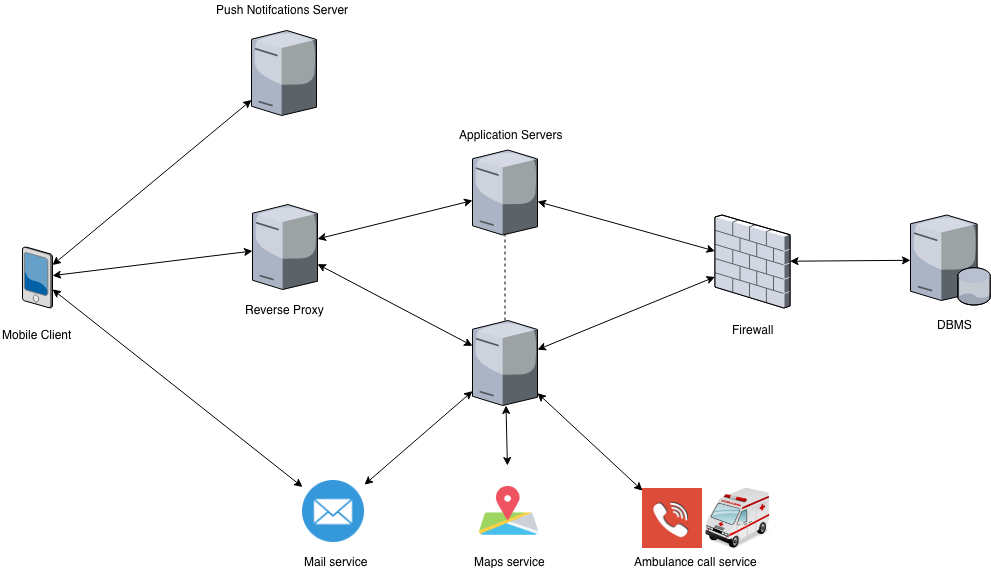
\includegraphics[width=\linewidth]{../images/design/OverviewDiagram.png}\\\\\\\\\\\\
		\end{figure}
		
		\item \textit{\textbf{Component view}}\\\\
		\begin{figure}[H]
		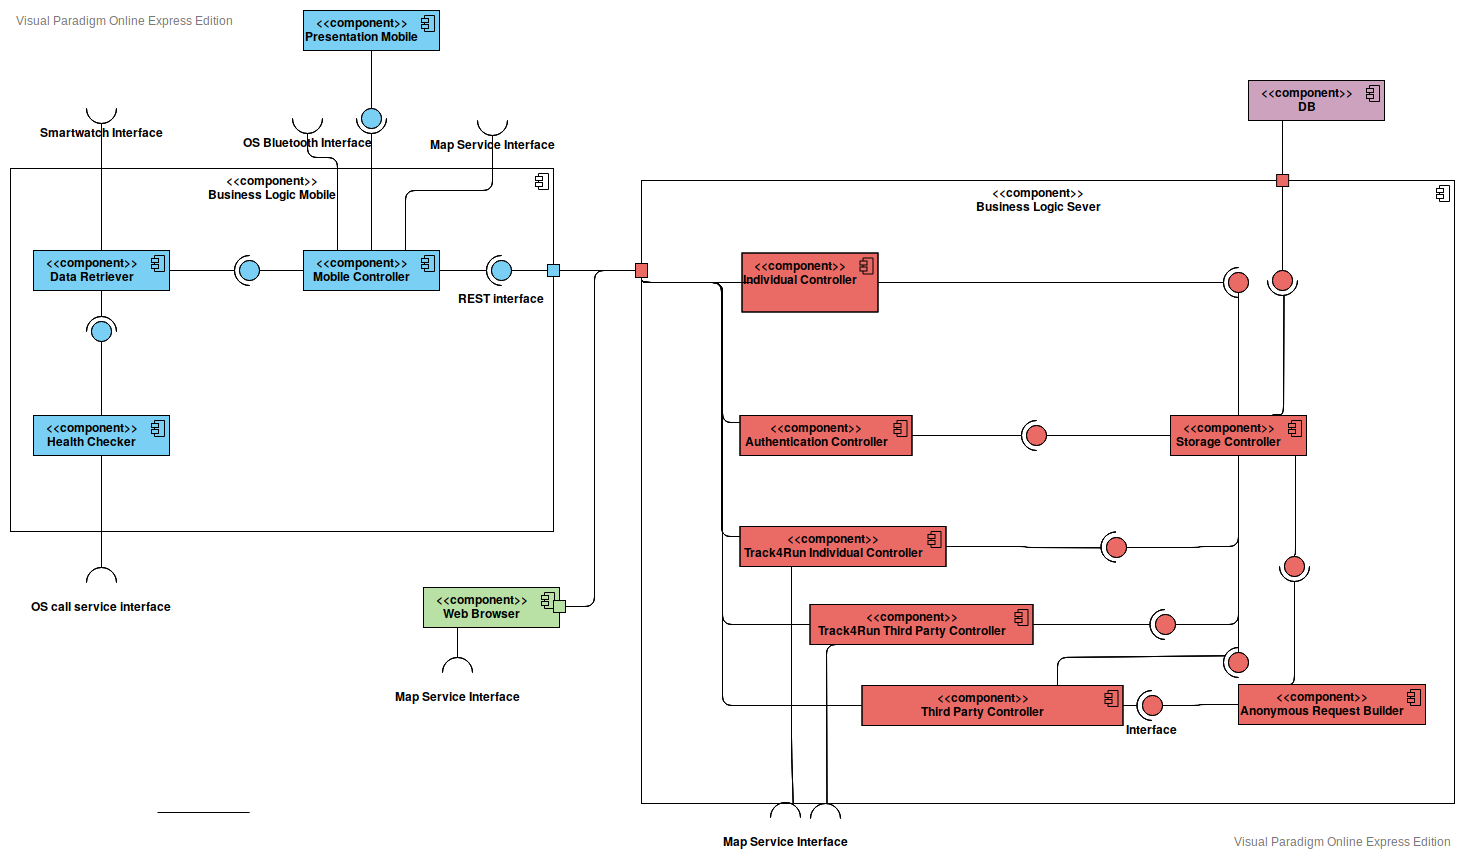
\includegraphics[width=\linewidth]{../images/design/ComponentDiagram.png}
		\end{figure}
		The UML component diagram shows the internal structure of the system highlighting the individual modules and the connections among them. It models the static implementation view of a system by breaking it down into various high levels of functionality.  Individual components are wired together by using an assembly connector to connect the required interface of one component with the provided interface of another component. For simplicity reasons, the interfaces between REST controllers (Individual, Third Party, Track4Run Individual and Track4Run Third Party Controller) and the Authentication Controller have not been drawn in the diagram. However they are present in the system in order to validate the successive user sessions after the log in. Below is the description of the components:\\
		\begin{itemize}
		\item{\textbf{Mobile Controller}\\
		This is the component that allows the individual mobile application to access to the API of the Business Logic Server. It implements the interface dedicated to the transfer of data from client to server and it translates the individual user interactions in REST API calls. If internet connection is not available or it's too slow, older health and location data are not saved locally but discarded by giving priority to new data.
				}\\
		\item{\textbf{Data Retriever}\\
		This component retrieves health data from smartwatches or similar devices, it filters them and forwards them to the Health Checker component, if the AutomatedSOS service is enabled, and to the Mobile Controller component.
				}\\
		\item{\textbf{Health Checker}\\
		This component analyzes in real time health data of the individual and checks if his or her health is fine. If it's not, it interacts with the operating system of the running application in order to make a SOS call.
				}\\
		\item{\textbf{Presentation}\\
		This is the component that is aimed to display the front-end content to the individual and to allow him or her to interact with the application.
				}\\
		\item{\textbf{Web Browser}\\
		The system allows the third party to interact with it through any web browser.
				}\\
		\item{\textbf{Router}\\
		It defines which controller entry points correspond to a given HTTP URL, and how parameters are to be read from the HTTP request.
				}\\
		\item{\textbf{Individual Controller}\\
		The main role of this component is to manage the data coming from the specific individual by invoking the proper methods of the Storage Controller. It also provides methods to accept/refuse a request of agreement and to change personal information or preferences. Furthermore it notifies the client if there are new requests or info for him.
				}\\
		\item{\textbf{Third Party Controller}\\
		This component provides methods that allow the third party to send invidual and anonymous requests to the system. If there are new individual agreements or new data available, it sends them to the third party.
				}\\
		\item{\textbf{Authentication Controller}\\
		This component provides authentication and registration processes for both the individuals and the third parties.
				}\\
		\item{\textbf{Track4Run Individual Controller}\\
		This component provides the methods to permit an individual to join, leave, check and watch a run. It communicates with the external service that provides maps through the Map services interface. Every time a user wants to join a run, it checks if all the constraints are satisfied (for example he can't join two overlapping runs). Finally, it keeps updated the individual about new info by sending him or her notifications.
				}\\
		\item{\textbf{Track4Run Third Party Controller}\\
		This component provides the methods to allow a third party to organize a run. It communicates with the external service that provides maps trough the Map services interface to allow the third party to select the track for the run.
				}\\				
		\item{\textbf{Storage Controller}
		This component provides the methods for querying and updating the Database.
				}\\
		\item{\textbf{Anonymous Request Builder}
		This component aggregates data in order to answer to third party group requests by assuring anonymity.
				}\\
		\item{\textbf{Database}
		This component represent the DBMS. It provides the interfaces to retrieve and store data. In the database there are data about users, third parties and the set of agreements among them. It also contains data about the runs.
				}\\
		\item{\textbf{External services interfaces}\\
		These interfaces are not implemented by the system but are provided by external services in order to run the application.
      	\begin{itemize}
		  	\item{\textbf{Map Service Interface}\\\
		  	It allows the third party to select the track and to show the position of runners in real time on the map.
						}\\
			\item{\textbf{OS Call Service Interface}\\
			It allows the mobile application to make a SOS phone call in case of emergency.
						}\\
			\item{\textbf{OS Bluetooth Interface}\\
			It allows the mobile application to connect the smartphone to smartwatches or similar devices.
						}\\
			\item{\textbf{Smartwatch Interface}\\
			It allows the mobile application to get data from smartwatches.
						}\\
      	\end{itemize}
				}
		\end{itemize}

		\item \textit{\textbf{Deployment view}}\\\\
		The figure below shows the deployment diagram of the whole system. Its main goal is to describe the distribution of components capturing the topology of the
system's hardware.\\
		\begin{figure}[H]
		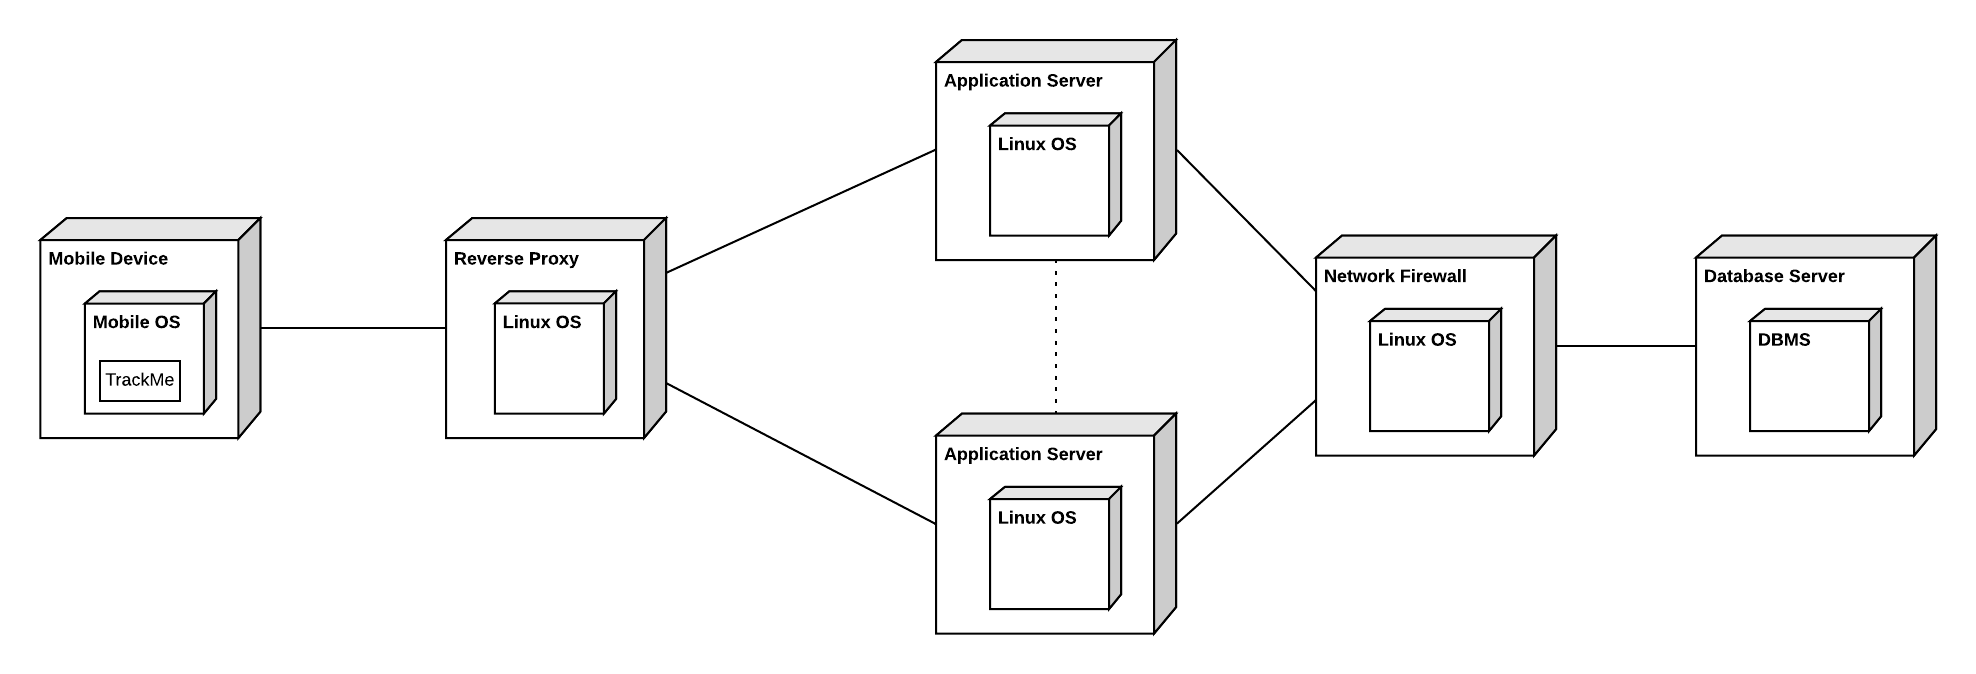
\includegraphics[width=\linewidth]{../images/design/DeploymentDiagram.png}\\
		\end{figure}
		As previously stated in the section 1, the system is structured in a multi-tier architecture. The specific role of each node is clarified here:\\\\
		\textbf{Clients}\\
The first tier is composed by the clients machines (mobile for individuals and desktop for third parties). The individuals will be able to access TrackMe functionalities through the dedicated native application while the third parties through any web browser.\\\\
		\textbf{Application Server}\\
This is the middleware level of the architecture: all the business logic of
the system is contained in this server.\\\\
		\textbf{Network Firewall}\\
The access to the Database is mediated by a network firewall in order to
avoid unauthorised access to the data and the credentials of the user.\\\\
		\textbf{Database Server}\\
This is the last layer of the architecture: all the data are stored in a Database Server accessed through a relational DBMS. \\\\
		\item \textit{\textbf{Runtime view}}\\
			\begin{legal}
				\item \textbf{Sign up Runtime View}\\
Third parties and individuals have to sign up to the application before being able to access its functionalities.
The registration process is the same for both third parties and individuals, the only thing that differentiates it  is the information provided by them.
The third party must fill up a form with its VAT number and a password. To reach the same goal an individual must fill up a form with username, password and personal data.
The information is serialized and then sent to the Application Server through an HTTP POST request.
The Authorization controller handles the request and, through the Storage interface, creates a new
entry in the User table or in the ThirdParty table on the Database. \\
				\begin{figure}[H]
				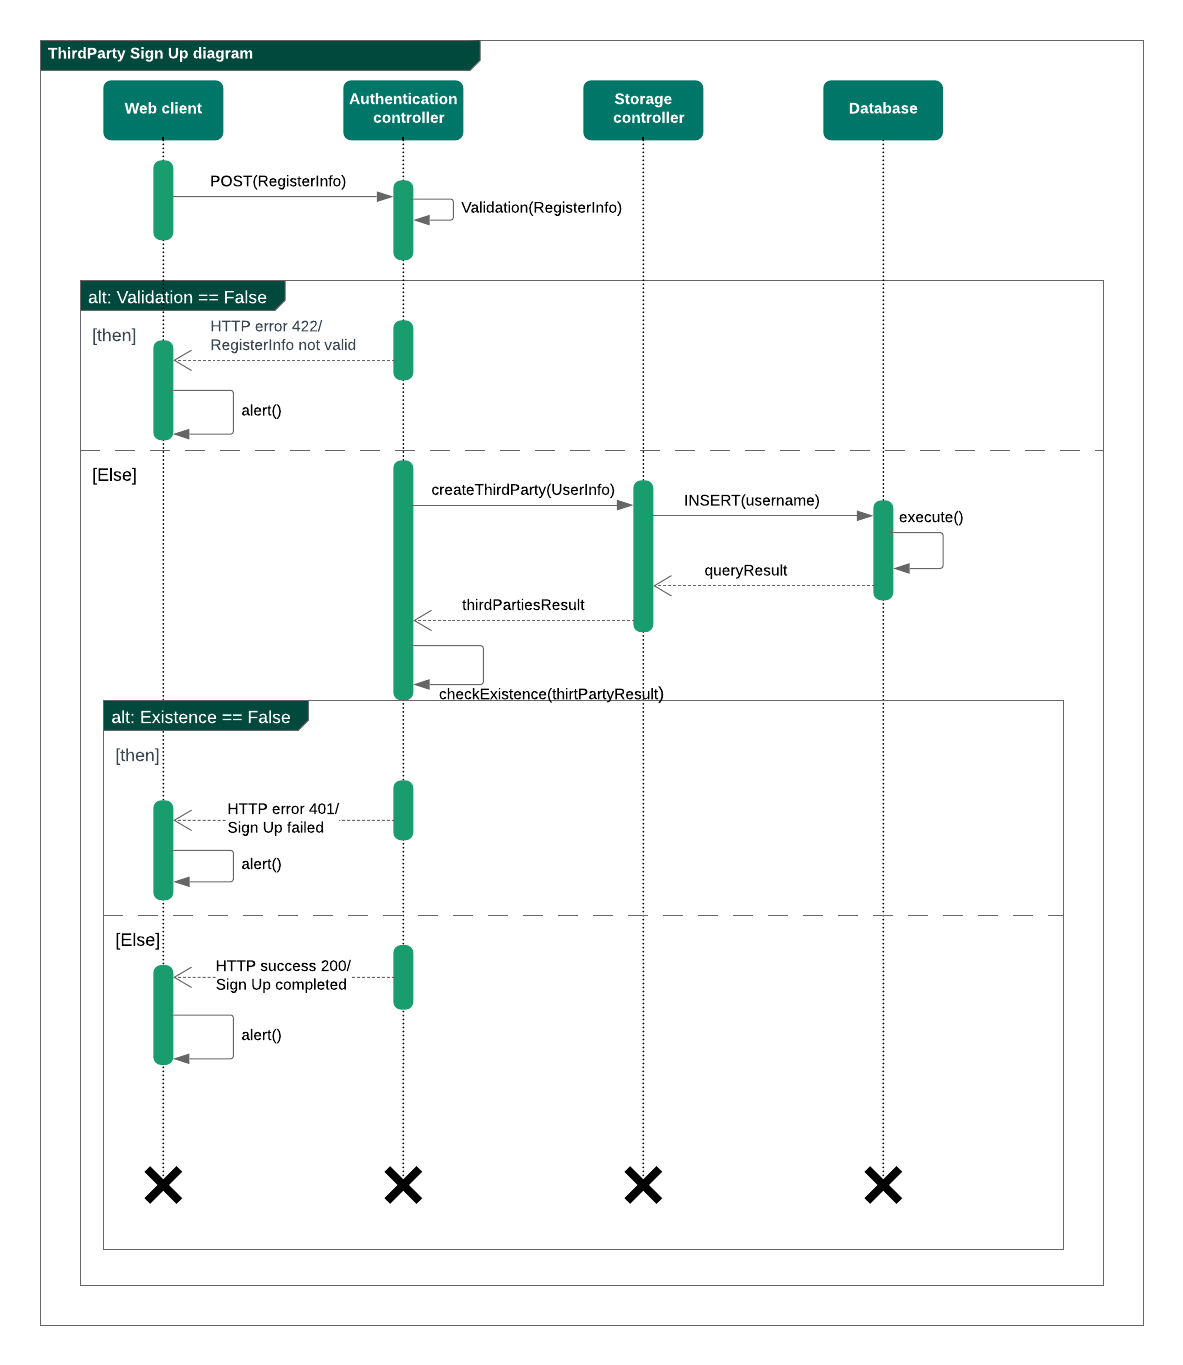
\includegraphics[width=\linewidth]{images/seq_diagrams/thirdPartySignUpSeq.png}\\
				\end{figure}
				
				\newpage
				\item \textbf{User Login Runtime View}\\
Third parties and individuals have to be logged to the application before being able to access its functionalities.
Both third parties and users submit the login information through and HTTP POST request.
The request is handled by the Authentication Controller that validates the request and checks if the Database has an entry for the requested account. If the entity is present and the credentials are correct, the Authentication Controller generates an Access Token, sets it as the current access Token for the specified entity and returns it to the entity itself.
The following sequence diagram shows how the process works in detail for the login of an individual user.\\
				\begin{figure}[H]
				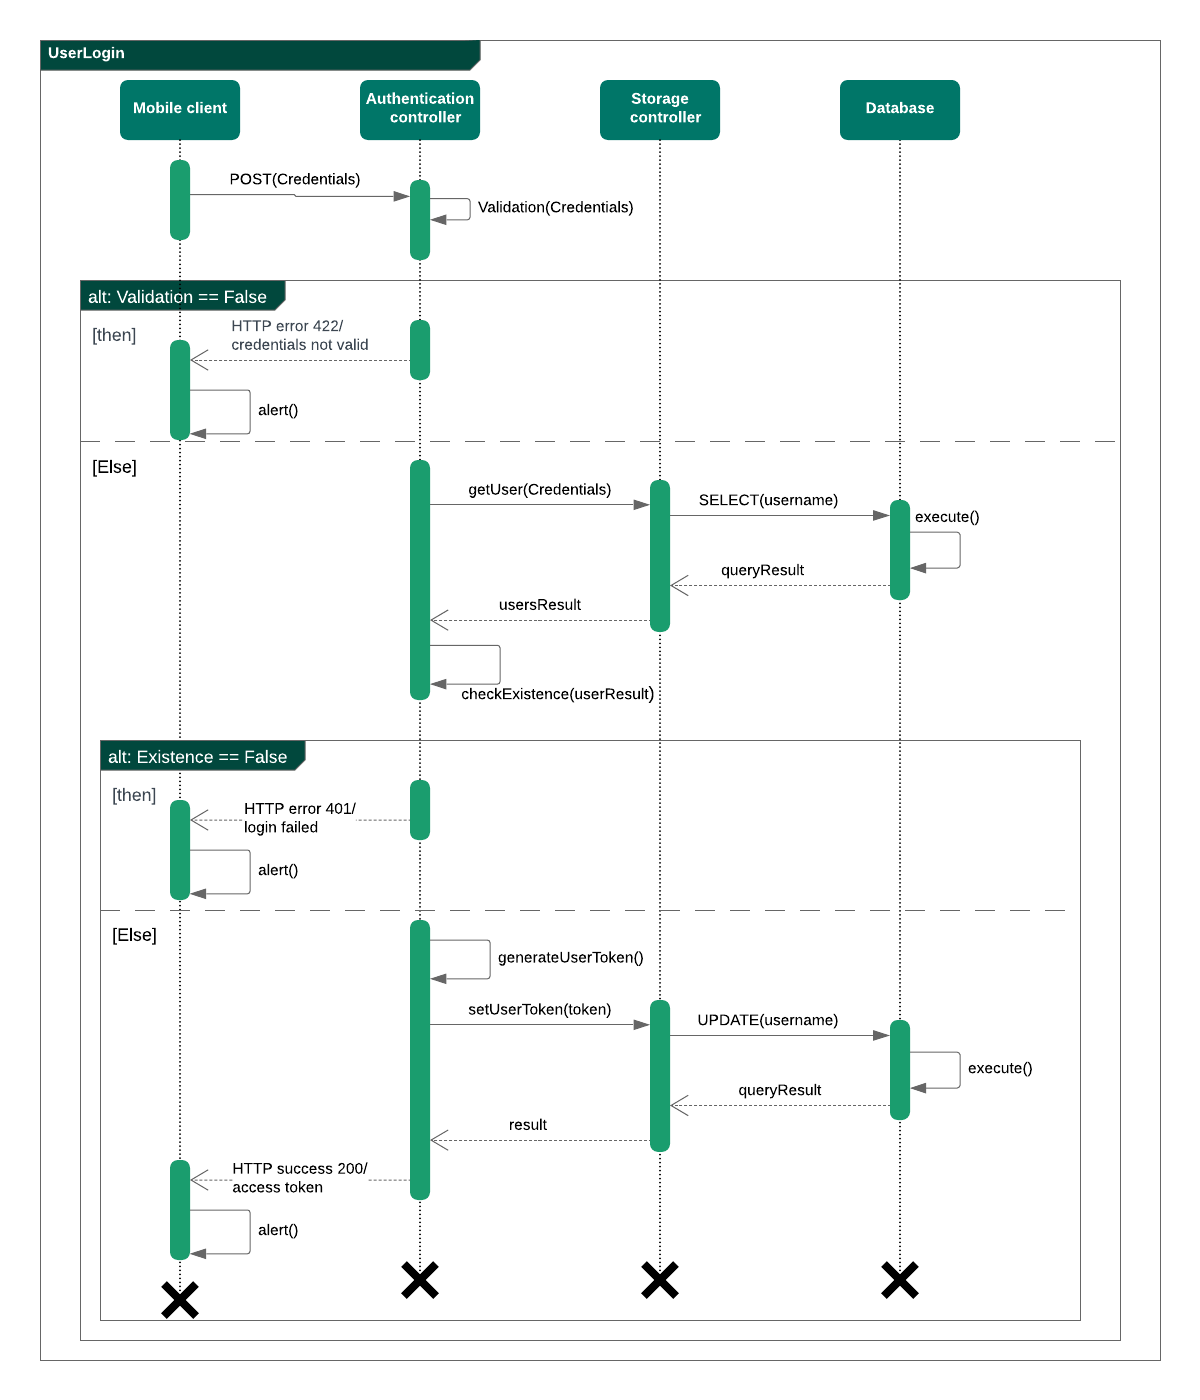
\includegraphics[width=\linewidth]{images/seq_diagrams/userLoginSeq.png}\\
				\end{figure}
				
				\newpage
				\item \textbf{Join a run Runtime View}\\
The User opens the Track4Run section of the application and, after a GET request to the Application Server he/she receives the list of all the available runs and he/she can choose to join one of them (if there is at least one displayed run).
The User can send a POST request containg the Access Token and the selected run to the Track4Run Individual Controller.
The Track4Run Individual Controller passes the Access Token to the Authentication Controller that checks if the Mobile Client provided a valid Token.
If the Authentication succeeds the control goes back to the Track4Run Individual Controller that checks if the user has already joined an overlapping run or if the maximum number of participants was reached.
If the control is satisfied the Track4Run Individual Controller asks the Storage Controller to update the tuple of the selected run in the Database.
To avoid repetitions, the following sequence diagram shows the process assuming that the User already received the list of available runs.
				\begin{figure}[H]
				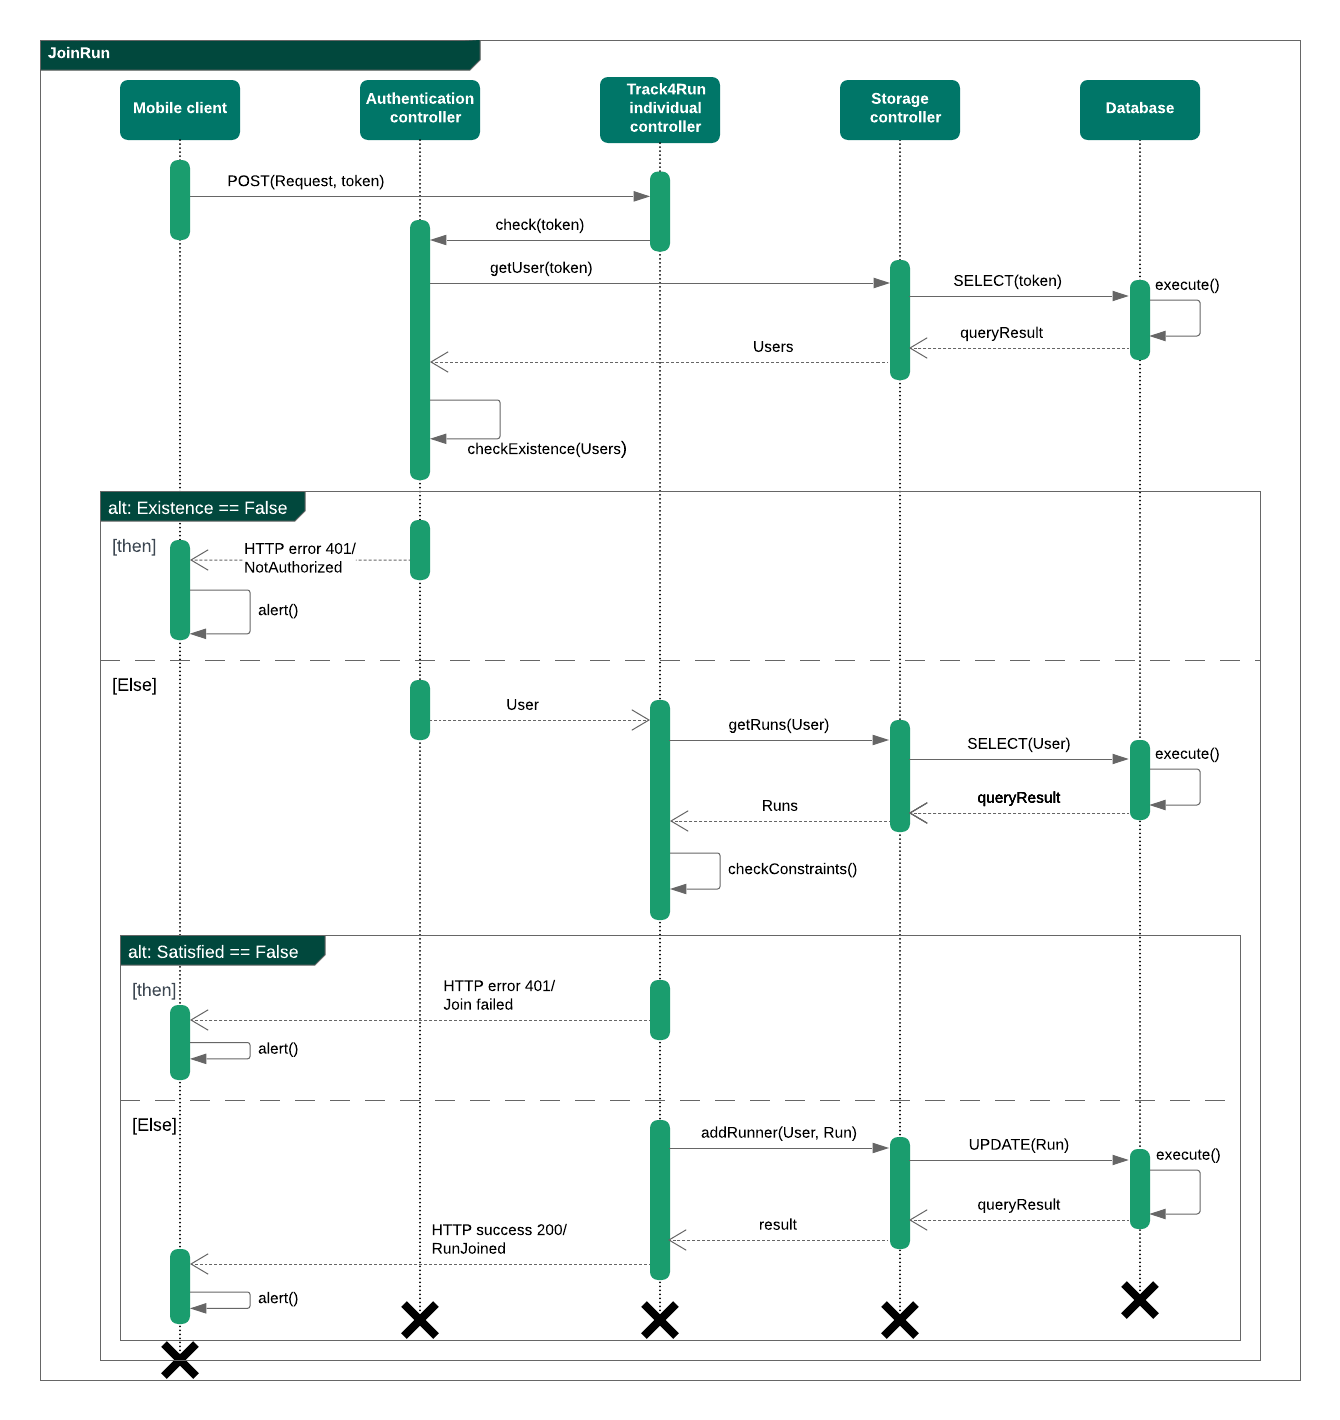
\includegraphics[width=\linewidth]{images/seq_diagrams/joinRunSeq.png}\\
				\end{figure}
				
				\newpage
				\item \textbf{Organise a run Runtime View}\\
The Third party opens the Track4Run section of the application and, after filling the form containing the information about the run it can send a POST request containg the Access Token and the filled form to the Track4Run Third Party Controller.
The Track4Run Third Party Controller passes the Access Token to the Authentication Controller that checks if the Web Client provided a valid Token.
If the Authentication succeeds the control goes back to the Track4Run Third Party Controller that asks the Storage Controller to insert a new tuple for the run in the Database.
				\begin{figure}[H]
				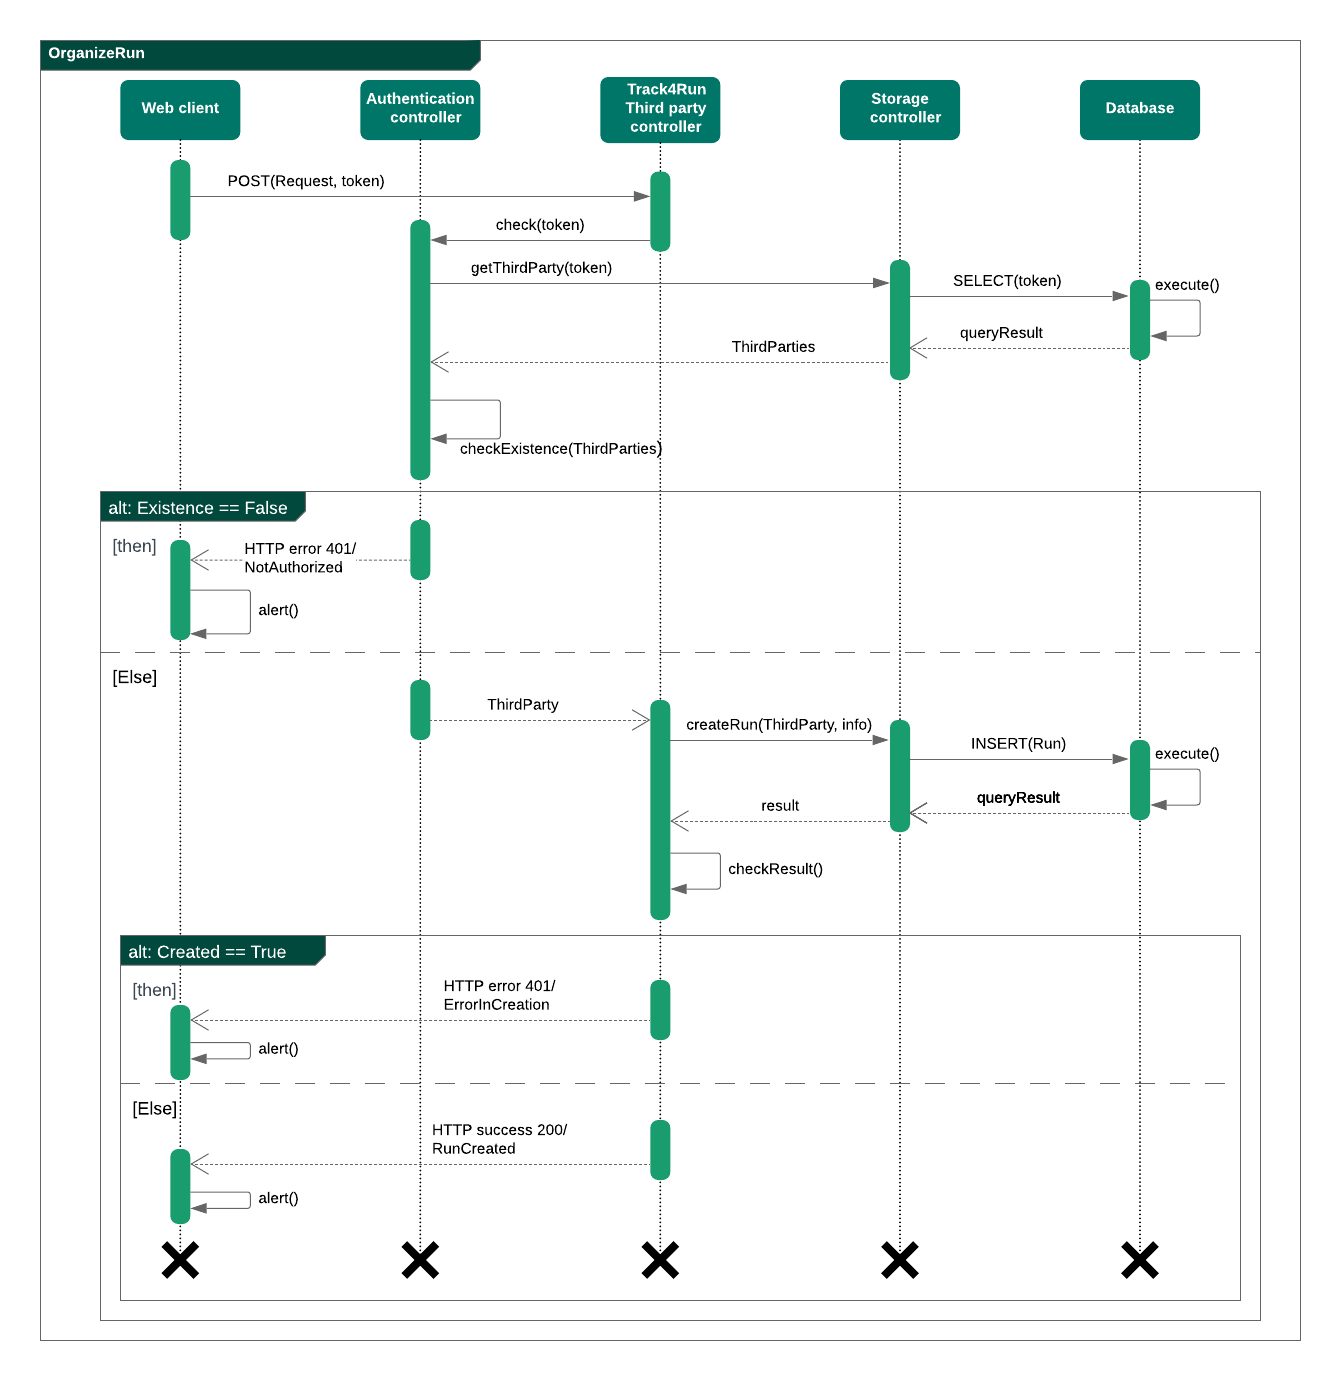
\includegraphics[width=\linewidth]{images/seq_diagrams/organizeRunSeq.png}\\
				\end{figure}
				
				\newpage
				\item \textbf{Individual request Runtime View}\\
				The Third party opens the Data4Help section of the application and, after filling the form containing the information about the request, it can send a POST request containg the Access Token and the filled form to the Third Party controller.
The Third Party Controller passes the Access Token to the Authentication Controller that checks if the Web Client provided a valid Token.
If the Authentication succeeds, the Third Party Controller forwards the request to the Storage Controller, that adds an instance of the request into the Database. Then, if the request is successfully inserted, the Third party is notified.
When this process is completed and the answer to the previous request is ready, the system will notify the Third Party as soon as it will ask for notifications.

				\begin{figure}[H]
				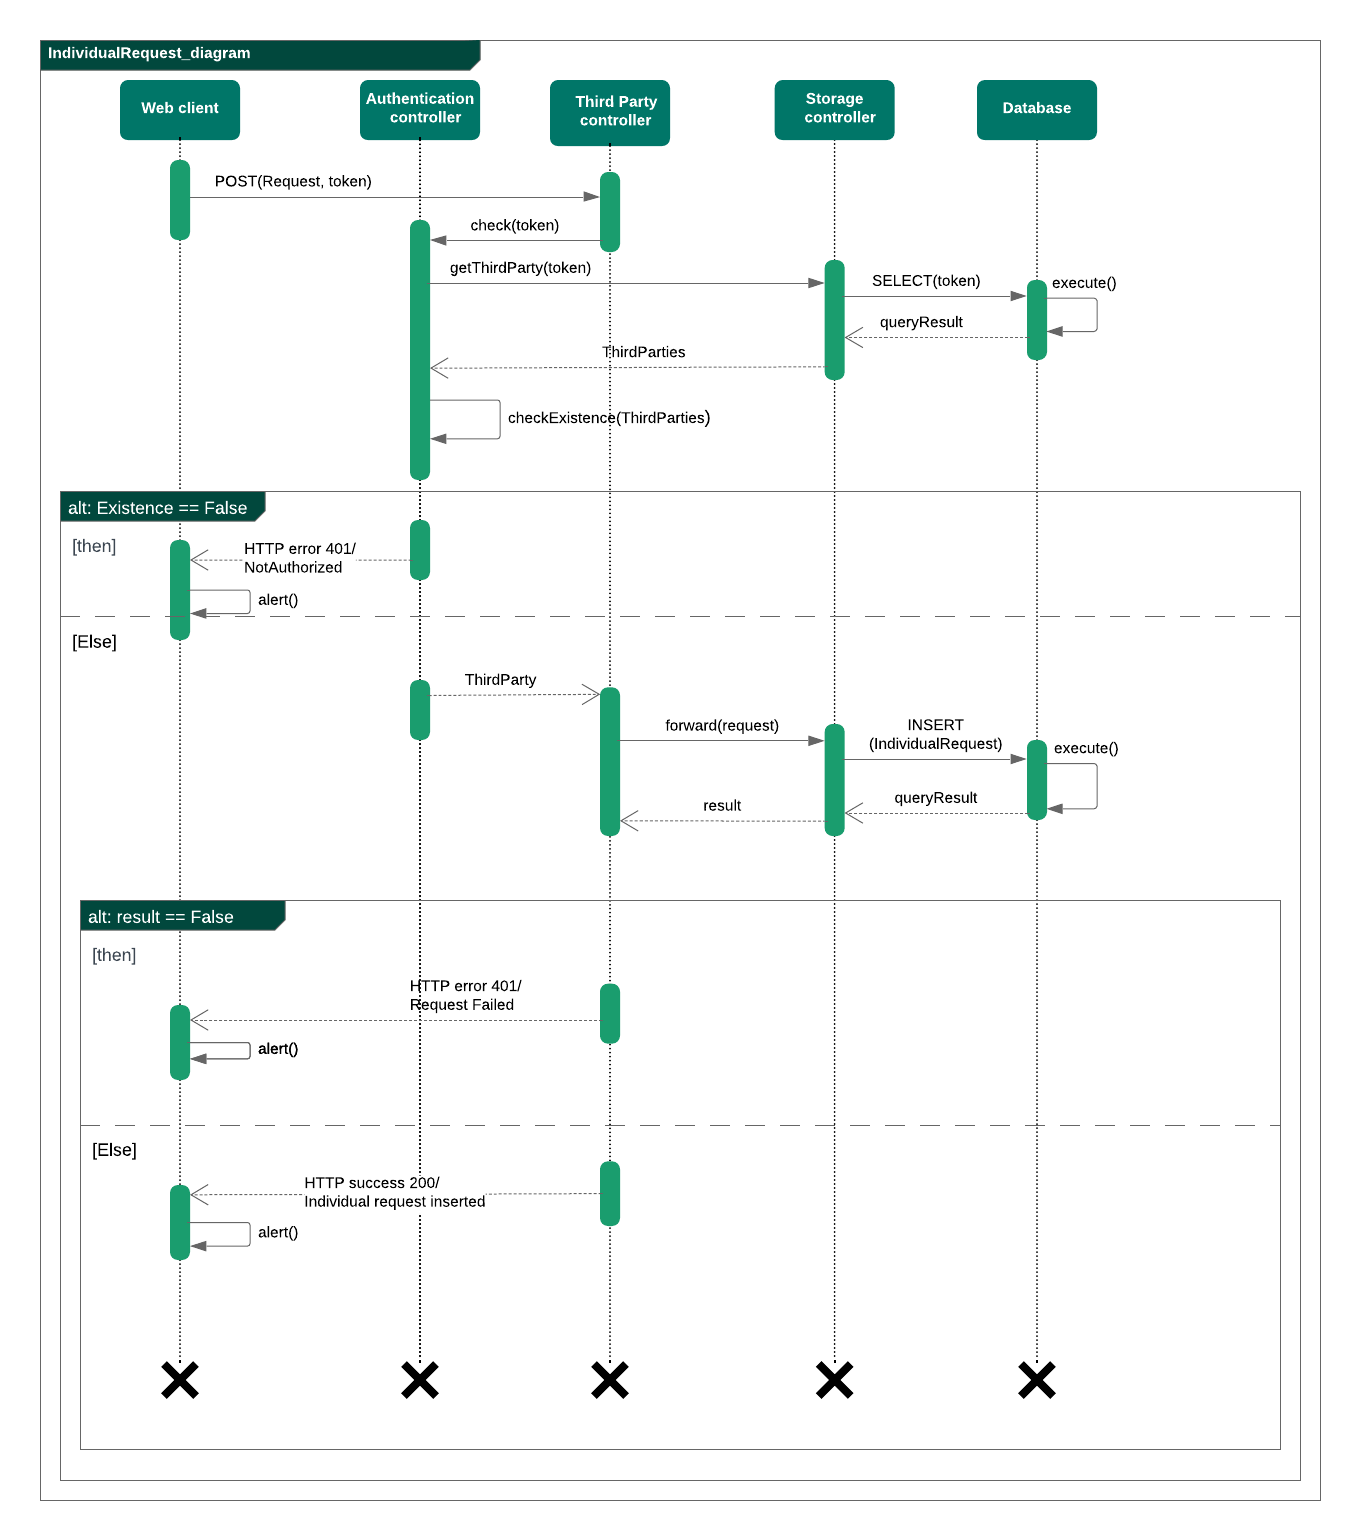
\includegraphics[width=\linewidth]{images/seq_diagrams/individualRequestSeq.png}\\
				\end{figure}
				
				\newpage
				\item \textbf{Group request Runtime View}\\
The Third party opens the Data4Help section of the application and, after filling the form containing the information about the request, it can send a POST request containg the Access Token and the filled form to the Third Party controller.
The Third Party Controller passes the Access Token to the Authentication Controller that checks if the Web Client provided a valid Token.
If the Authentication succeeds, the Third Party Controller asks the Anonymuos Request Builder to get the data from the Database, through the Storage Controller. If the constraints on data are satisfied, the Third Party Controller asks the Storage Controller to add an instance of the request into the Database. Then, if the request is successfully inserted, the Third party is notified and the Third Party Controller communicates the Anonymous Request Builder to aggregate the received data.
				\begin{center}
				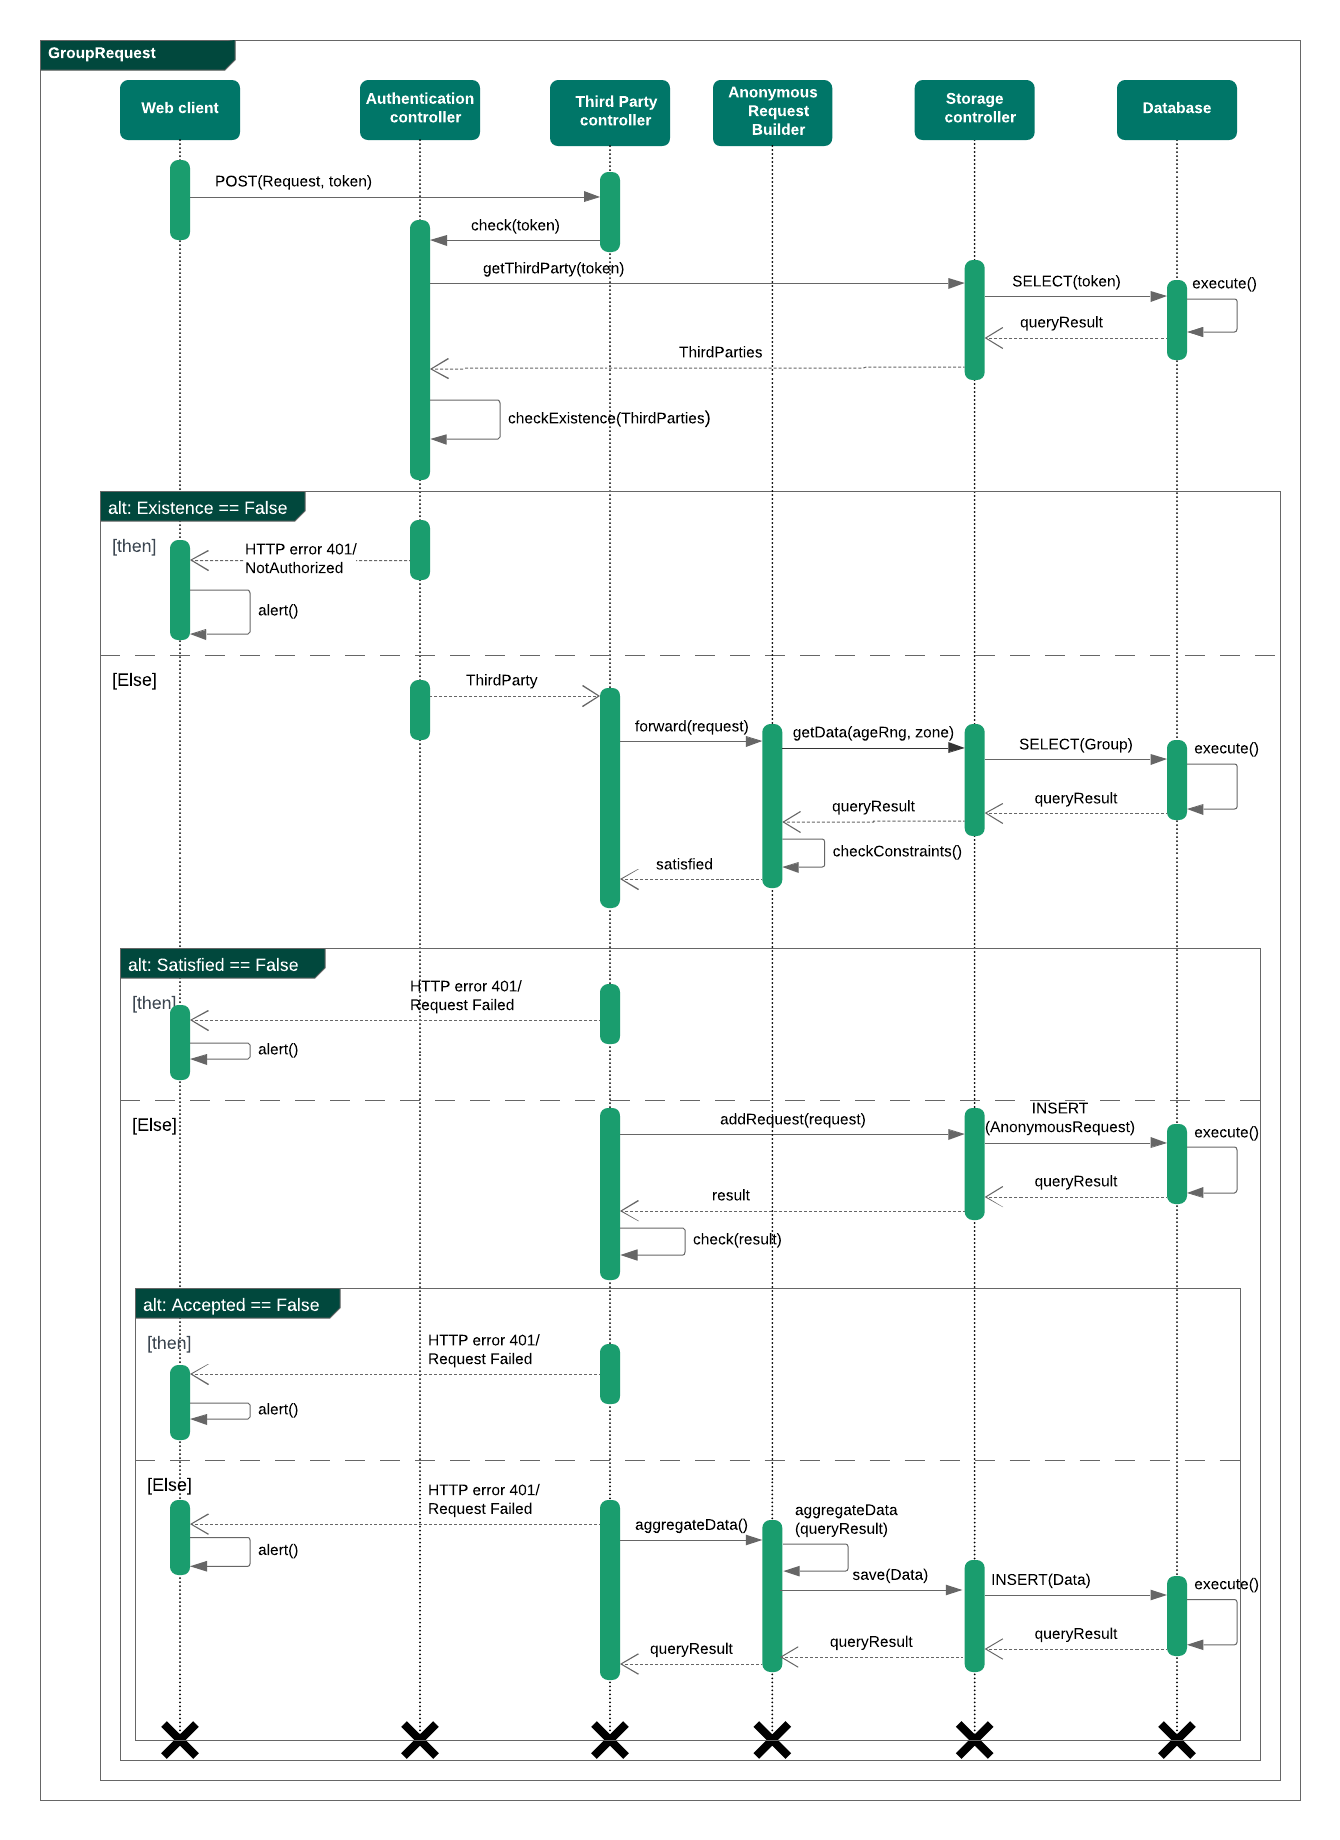
\includegraphics[width=14cm]{images/seq_diagrams/groupRequestSeq.png}\\
				\end{center}
				
				\newpage
				\item \textbf{AutomatedSOS Runtime View}\\
				This runtime view shows the interactions among mobile client components, from the retrieving of data, from the smartwatch, to the eventual SOS call.
				\begin{figure}[H]
				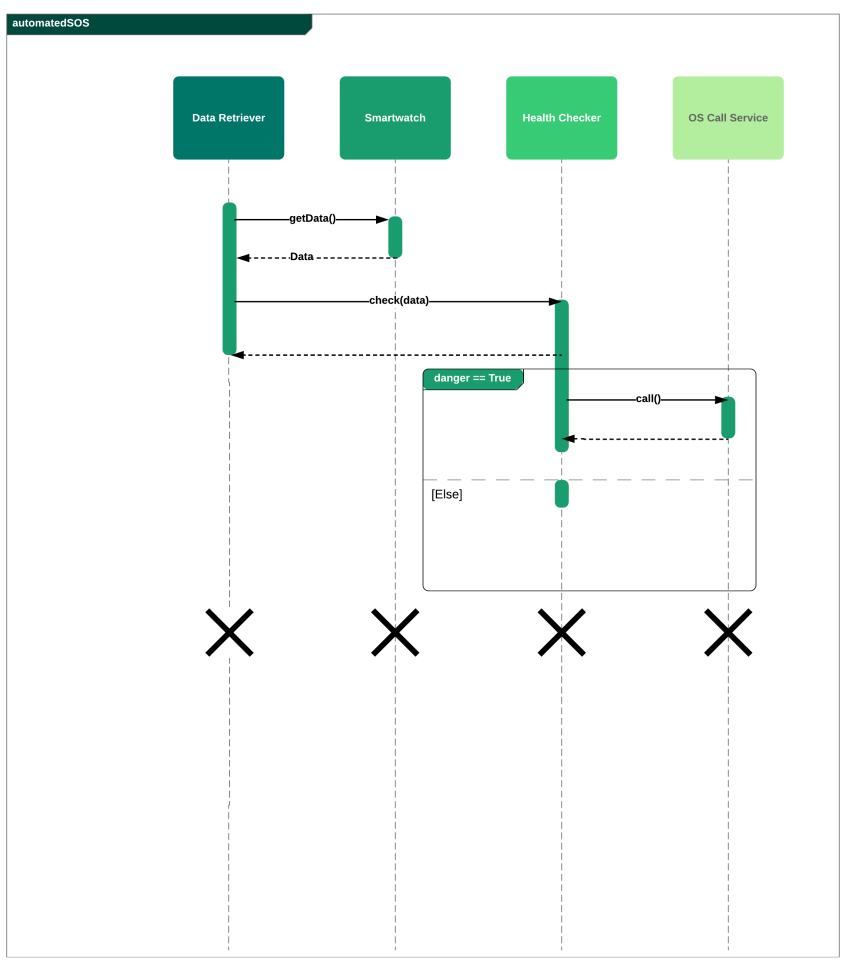
\includegraphics[width=\linewidth]{images/seq_diagrams/automatedSOSSeq.png}\\
				\end{figure}
			\end {legal}
		\newpage
		\item \textit{\textbf{Component interfaces}}\\\\
			\begin{legal} 
				\item \textit{\textbf{REST API}}\\\\
				REST (REpresentation State Transfer) describes an architectural style of networked systems such as this application. One of the most important REST principles for Web applications is that the interaction between the client and server is stateless between requests. Each request from the client to the server must contain all of the information necessary to understand the request. The client wouldn't notice if the server were to be restarted at any point between the requests. Additionally, stateless requests are free to be answered by any available server, which is appropriate for an environment such as cloud computing. On the server side, the application state and functionality are divided into resources. A resource is an item of interest, a conceptual identity that is exposed to the clients. Every resource is uniquely addressable using a URI (Universal Resource Identifier). All resources share a uniform interface for the transfer of state between client and server. Standard HTTP methods such as GET, PUT, POST, and DELETE are used. Hypermedia is the engine of the application state, and resource representations are interconnected by hyperlinks, as described partially in this section and section 3.\\

					\begin{itemize}
						\item \textbf{Authentication Controller} \\
						
						\textbf{Third Party SignUp} \\
						
							\begin{tabularx}{\linewidth}{| l| l }
								\hline
								endpoint & */auth/thirdparty/signUp \\
								\hline
								method & POST \\
								\hline
								url params & \\
								\hline
								data params &
								\parbox{0.7\textwidth}{
									\bigskip
									VAT: [alphanumeric]\\
									name: [alphanumeric]\\
									password : [alphanumeric]
									\bigskip
								} \\
								\hline
								success response &
								\parbox{0.7\textwidth}{
									\bigskip
									code: 200\\
								} \\
								\hline
								error response &
								\parbox{0.7\textwidth}{
									\bigskip
									code: 400 BAD REQUEST \\
									Content : \{error: "JSON parse error"\}\\
									code: 500 INTERNAL SERVER ERROR \\
									Content : \{error: "Could not commit JPA transaction"\}\\
									code: 409 CONFLICT \\
									Content : \{error: "This user already exists"\}
									\bigskip
								} \\
								\hline
								Notes & 
								\parbox{0.7\textwidth}{
									\bigskip Allows a third party to register to the system.
								\bigskip}  \\
								\hline
							\end{tabularx}\\
							
						\newpage
						\textbf{Individual SignUp} \\
			
							\begin{tabularx}{\linewidth}{| l| l }
								\hline
								endpoint & */auth/individual/signUp \\
								\hline
								method & POST \\
								\hline
								url params & \\
								\hline
								data params &
								\parbox{0.7\textwidth}{
									\bigskip
									username: [alphanumeric]\\
									password : [alphanumeric]\\
									name: [text]\\
									surname: [text]\\
									latitude: [numeric]\\
									longitude: [numeric]\\
									birthDate: [date]
									\bigskip
								} \\
								\hline
								success response &
								\parbox{0.7\textwidth}{
									\bigskip
									code: 200\\
								} \\
								\hline
								error response &
								\parbox{0.7\textwidth}{
									\bigskip
									code: 400 BAD REQUEST \\
									Content : \{error: "JSON parse error"\}\\
									code: 500 INTERNAL SERVER ERROR \\
									Content : \{error: "Could not commit JPA transaction"\}\\
									code: 409 CONFLICT \\
									Content : \{error: "This user already exists"\}
									\bigskip
								} \\
								\hline
								Notes & 
								\parbox{0.7\textwidth}{
									\bigskip Allows an individual to register to the system.
								\bigskip}  \\
								\hline
							\end{tabularx}\\\\
					
							\textbf{Login}\\

								\begin{tabularx}{\linewidth}{| l| l }
									\hline
									endpoint & */auth\\
									\hline
									method & POST \\
									\hline
									url params & \\
									\hline
									data params &
									\parbox{0.7\textwidth}{
										\bigskip
										username: [alphanumeric]\\
										password : [alphanumeric]
										\bigskip
									} \\
									\hline
									success response &
									\parbox{0.7\textwidth}{
										\bigskip
										code: 200\\
										Content : \{token: [alphanumeric]\}
										\bigskip
									} \\
									\hline
									error response &
									\parbox{0.7\textwidth}{
										\bigskip
										code: 400 BAD REQUEST \\
										Content : \{error: "JSON parse error"\}\\
										Code: 401 UNAUTHORIZED \\
										Content : \{error: "Bad Credentials!"\}
										\bigskip
									} \\
									\hline
									Notes & 
									\parbox{0.7\textwidth}{
										\bigskip Allows an individual or a third party to obtain an authentication Token
									\bigskip }\\
									\hline
								\end{tabularx}\\
							\newpage
							
							\textbf{NOTE: }
							\begin{itemize}
							\item all successive requests need to contain the token, retrieved during the login request, in order to be allowed;
							\item if a logged in user try to use REST API trying to be another user a excepction is launched (code: 401 UNAUTHORIZED Content : \{error: "Trying to be another user!"\}.
							\end{itemize}
							\item \textbf{Third Party Controller} \\
					
							\textbf{Make and individual request} \\
			
							\begin{tabularx}{\linewidth}{| l| l }
								\hline
								endpoint & *thirdparty/individualRequest \\
								\hline
								method & POST \\
								\hline
								url params & \\
								\hline
								data params &
								\parbox{0.7\textwidth}{
									\bigskip
									vat: [alphanumeric]\\
									fiscalcode: [alphanumeric]\\
									subscribedToNewData: [boolean]
									\bigskip
								} \\
								\hline
								success response &
								\parbox{0.7\textwidth}{
									\bigskip
									code: 200
									\bigskip
								} \\
								\hline
								error response &
								\parbox{0.7\textwidth}{
									\bigskip
									code: 400 BAD REQUEST \\
									Content : \{error: "JSON parse error"\}\\
									code: 409 CONFLICT \\
									Content : \{error: "This user already exists"\}\\
									code: 401 UNAUTHORIZED \\
									Content : \{error: "Bad credentials!"\}\\
									code: 404 NOT FOUND \\
									Content : \{error: "Third Party Not Found"\}\\
									code: 404 NOT FOUND \\
									Content : \{error: "Individual Not Found"\}\\
									Code: 401 CONFLICT \\
									Content : \{error: ""This request has been already done""\}\\
									\bigskip
								} \\
								\hline
								Notes & 
								\parbox{0.7\textwidth}{
									\bigskip Allows the third party to do an individual request of data.
								\bigskip}  \\
								\hline
							\end{tabularx}\\
							\newpage
							\textbf{Make and anonymous request} \\
			
							\begin{tabularx}{\linewidth}{| l| l }
								\hline
								endpoint & *thirdparty/anonymousRequest \\
								\hline
								method & POST \\
								\hline
								url params & \\
								\hline
								data params &
								\parbox{0.7\textwidth}{
									\bigskip
									vat: [alphanumeric]\\
									startAge: [numeric]\\
									endAge: [numeric]\\
									lat1: [float]\\
									lon1: [float]\\
									lat2: [float]\\
									lon2: [float]\\
									subscribedToNewData: [boolean]
									\bigskip
								} \\
								\hline
								success response &
								\parbox{0.7\textwidth}{
									\bigskip
									code: 200
									\bigskip
								} \\
								\hline
								error response &
								\parbox{0.7\textwidth}{
									\bigskip
									code: 400 BAD REQUEST \\
									Content : \{error: "JSON parse error"\}\\
									code: 500 INTERNAL SERVER ERROR \\
									Content : \{error: "Could not commit JPA transaction"\}\\
									code: 401 UNAUTHORIZED \\
									Content : \{error: "Bad credentials!"\}\\
									code: 404 NOT FOUND \\
									Content : \{error: "Third Party Not Found"\}\\
									\bigskip
								} \\
								\hline
								Notes & 
								\parbox{0.7\textwidth}{
									\bigskip Allows the third party to do a group request of data.
								\bigskip}  \\
								\hline
							\end{tabularx}\\\\
					
							\textbf{Modify Third Party Password}\\
				
							\begin{tabularx}{\linewidth}{| l| l }
								\hline
								endpoint & */thirdParty/{username}/changePassword \\
								\hline
								method & PUT \\
								\hline
								url params & 
								\parbox{0.7\textwidth}{
									\bigskip
									username: [alphanumeric]
									\bigskip
								}\\
								\hline
								data params & 
								\parbox{0.7\textwidth}{
									\bigskip
									newPassword: [alphanumeric]\\
									oldPassword:[alphanumeric]
									\bigskip
								} \\
								\hline
								success response &
								\parbox{0.7\textwidth}{
									\bigskip
									Code: 200
									\bigskip
								} \\
								\hline
								error response &
								\parbox{0.7\textwidth}{
									\bigskip
									code: 400 BAD REQUEST \\
									Content : \{error: "JSON parse error"\}\\
									code: 401 UNAUTHORIZED \\
									Content : \{error: "Bad credentials!"\}\\
									code: 404 NOT FOUND \\
									Content : \{error: "Third Party Not Found"\}\\
									code: 422 UNPROCESSABLE ENTITY\\
									Content : \{error: "Bad Credentials"\}\\
									code: 422 UNPROCESSABLE ENTITY\\
									Content : \{error: "Data are not well formed"\}
									\bigskip
								} \\
								\hline
								Notes & \parbox{0.7\textwidth}{
									\bigskip
									Allows a third party to change its password.
									\bigskip
								} \\
								\hline
							\end{tabularx}\\
							\newpage
							\textbf{Get individual requests} \\
			
								\begin{tabularx}{\linewidth}{| l| l }
									\hline
									endpoint & */thirdParty/\{thirdParty\}/individualRequests \\
									\hline
									method & GET \\
									\hline
									data params & \\
									\hline
									url params &
									\parbox{0.7\textwidth}{
										\bigskip
										vat: [alphanumeric]
										\bigskip
									} \\
									\hline
									success response &
									\parbox{0.7\textwidth}{
										\bigskip
										code: 200\\
										Content : \{individualRequests: List<IndividualRequest>\}
										\bigskip
									} \\
									\hline
									error response &
									\parbox{0.7\textwidth}{
										\bigskip
										code: 400 BAD REQUEST \\
										Content : \{error: "JSON parse error"\}\\
										code: 401 UNAUTHORIZED \\
										Content : \{error: "Bad credentials!"\}\\
										code: 404 NOT FOUND \\
										Content : \{error: "Third Party Not Found"\}
										\bigskip
									} \\
									\hline
									Notes & 
									\parbox{0.7\textwidth}{
										\bigskip Allows the third parties to request for all individual requests it has done.
									\bigskip}  \\
									\hline
								\end{tabularx}\\\\
								
								\textbf{Get individual request notifications} \\
			
								\begin{tabularx}{\linewidth}{| l| l }
									\hline
									endpoint & */thirdParty/\{thirdParty\}/notifications/individualRequests \\
									\hline
									method & GET \\
									\hline
									data params & \\
									\hline
									url params &
									\parbox{0.7\textwidth}{
										\bigskip
										vat: [alphanumeric]
										\bigskip
									} \\
									\hline
									success response &
									\parbox{0.7\textwidth}{
										\bigskip
										code: 200\\
										Content : \{notifications: List<IndividualRequest>\}
										\bigskip
									} \\
									\hline
									error response &
									\parbox{0.7\textwidth}{
										\bigskip
										code: 400 BAD REQUEST \\
										Content : \{error: "JSON parse error"\}\\
										code: 401 UNAUTHORIZED \\
										Content : \{error: "Bad credentials!"\}\\
										code: 404 NOT FOUND \\
										Content : \{error: "Third Party Not Found"\}
										\bigskip
									} \\
									\hline
									Notes & 
									\parbox{0.7\textwidth}{
										\bigskip Allows the third parties to request for notifications of individual requests.
									\bigskip}  \\
									\hline
								\end{tabularx}\\\\
								
								\textbf{Get individual request notifications counter} \\
			
								\begin{tabularx}{\linewidth}{| l| l }
									\hline
									endpoint & */thirdParty/\{thirdParty\}/notifications/countIndividualRequests \\
									\hline
									method & GET \\
									\hline
									data params & \\
									\hline
									url params &
									\parbox{0.7\textwidth}{
										\bigskip
										vat: [alphanumeric]
										\bigskip
									} \\
									\hline
									success response &
									\parbox{0.7\textwidth}{
										\bigskip
										code: 200\\
										Content : \{counter: [integer]\}
										\bigskip
									} \\
									\hline
									error response &
									\parbox{0.7\textwidth}{
										\bigskip
										code: 400 BAD REQUEST \\
										Content : \{error: "JSON parse error"\}\\
										code: 401 UNAUTHORIZED \\
										Content : \{error: "Bad credentials!"\}\\
										code: 404 NOT FOUND \\
										Content : \{error: "Third Party Not Found"\}
										\bigskip
									} \\
									\hline
									Notes & 
									\parbox{0.7\textwidth}{
										\bigskip Allows the third parties to request for the number of new notifications of individual requests.
									\bigskip}  \\
									\hline
								\end{tabularx}\\\\
								
								\textbf{Get past individual data} \\
			
								\begin{tabularx}{\linewidth}{| l| l }
									\hline
									endpoint & */thirdParty/\{thirdParty\}/\{individual\}/data \\
									\hline
									method & GET \\
									\hline
									data params & \\
									\hline
									url params &
									\parbox{0.7\textwidth}{
										\bigskip
										vat: [alphanumeric]\\
										fiscalCode: [alphanumeric]
										\bigskip
									} \\
									\hline
									success response &
									\parbox{0.7\textwidth}{
										\bigskip
										code: 200\\
										Content : \{individual data: List$<$IndividualData$>$\}
										\bigskip
									} \\
									\hline
									error response &
									\parbox{0.7\textwidth}{
										\bigskip
										code: 400 BAD REQUEST \\
										Content : \{error: "JSON parse error"\}\\
										code: 401 UNAUTHORIZED \\
										Content : \{error: "Bad credentials!"\}\\
										code: 404 NOT FOUND \\
										Content : \{error: "Third Party Not Found"\}\\
										code: 404 NOT FOUND \\
										Content : \{error: "Individual Not Found"\}\\
										code: 404 NOT FOUND \\
										Content : \{error: "The thirdParty has not the right to receive data from the individual because you never asked for it"\}\\
										code: 400 BAD REQUEST \\
										Content : \{error: "You can't acces this data"\}\\
										\bigskip
									} \\
									\hline
									Notes & 
									\parbox{0.7\textwidth}{
										\bigskip Allows the third parties to request for past data of a specific individual.
									\bigskip}  \\
									\hline
								\end{tabularx}\\
								
								\textbf{Get new individual data} \\
			
								\begin{tabularx}{\linewidth}{| l| l }
									\hline
									endpoint & */thirdParty/\{thirdParty\}/notifications/\{individual\} \\
									\hline
									method & GET \\
									\hline
									data params & \\
									\hline
									url params &
									\parbox{0.7\textwidth}{
										\bigskip
										vat: [alphanumeric]\\
										fiscalCode: [alphanumeric]
										\bigskip
									} \\
									\hline
									success response &
									\parbox{0.7\textwidth}{
										\bigskip
										code: 200\\
										Content : \{notifications: List$<$IndividualData$>$\}
										\bigskip
									} \\
									\hline
									error response &
									\parbox{0.7\textwidth}{
										\bigskip
										code: 400 BAD REQUEST \\
										Content : \{error: "JSON parse error"\}\\
										code: 401 UNAUTHORIZED \\
										Content : \{error: "Bad credentials!"\}\\
										code: 404 NOT FOUND \\
										Content : \{error: "Third Party Not Found"\}\\
										code: 404 NOT FOUND \\
										Content : \{error: "Individual Not Found"\}\\
										code: 404 NOT FOUND \\
										Content : \{error: "The thirdParty has not the right to receive data from the individual because you never asked for it"\}\\
										code: 400 BAD REQUEST \\
										Content : \{error: "You can't acces this data"\}\\
										\bigskip
									} \\
									\hline
									Notes & 
									\parbox{0.7\textwidth}{
										\bigskip Allows the third parties to request for new data of a specific individual.
									\bigskip}  \\
									\hline
								\end{tabularx}\\
								
								\textbf{Get anonymous requests} \\
			
								\begin{tabularx}{\linewidth}{| l| l }
									\hline
									endpoint & */thirdParty/\{thirdParty\}/anonymousRequests \\
									\hline
									method & GET \\
									\hline
									data params & \\
									\hline
									url params &
									\parbox{0.7\textwidth}{
										\bigskip
										vat: [alphanumeric]
										\bigskip
									} \\
									\hline
									success response &
									\parbox{0.7\textwidth}{
										\bigskip
										code: 200\\
										Content : \{anonymousRequests: List$<$AnonymousRequest$>$\}
										\bigskip
									} \\
									\hline
									error response &
									\parbox{0.7\textwidth}{
										\bigskip
										code: 400 BAD REQUEST \\
										Content : \{error: "JSON parse error"\}\\
										code: 401 UNAUTHORIZED \\
										Content : \{error: "Bad credentials!"\}\\
										code: 404 NOT FOUND \\
										Content : \{error: "Third Party Not Found"\}
										\bigskip
									} \\
									\hline
									Notes & 
									\parbox{0.7\textwidth}{
										\bigskip Allows the third parties to request for all anonymous requests it has done.
									\bigskip}  \\
									\hline
								\end{tabularx}\\\\
								
								\textbf{Get past anonymous request data} \\
			
								\begin{tabularx}{\linewidth}{| l| l }
									\hline
									endpoint & */thirdParty/\{thirdParty\}/anonymousAnswer/\{anonymousAnswer\} \\
									\hline
									method & GET \\
									\hline
									data params & \\
									\hline
									url params &
									\parbox{0.7\textwidth}{
										\bigskip
										vat: [alphanumeric]\\
										anonymousRequestId: [alphanumeric]
										\bigskip
									} \\
									\hline
									success response &
									\parbox{0.7\textwidth}{
										\bigskip
										code: 200\\
										Content : \{anonymous answers: List$<$AnonymousAnswer$>$\}
										\bigskip
									} \\
									\hline
									error response &
									\parbox{0.7\textwidth}{
										\bigskip
										code: 400 BAD REQUEST \\
										Content : \{error: "JSON parse error"\}\\
										code: 401 UNAUTHORIZED \\
										Content : \{error: "Bad credentials!"\}\\
										code: 404 NOT FOUND \\
										Content : \{error: "Third Party Not Found"\}\\
										code: 404 NOT FOUND \\
										Content : \{error: "Anonymous Request Not Found"\}\\
										code: 400 BAD REQUEST \\
										Content : \{error: "Not your request"\}\\
										\bigskip
									} \\
									\hline
									Notes & 
									\parbox{0.7\textwidth}{
										\bigskip Allows the third parties to request for past data of an anonymous request.
									\bigskip}  \\
									\hline
								\end{tabularx}\\
								
								\textbf{Get new anonymous request data} \\
			
								\begin{tabularx}{\linewidth}{| l| l }
									\hline
									endpoint & */thirdParty/\{thirdParty\}/anonymousAnswer/notifications/\{anonymousAnswer\} \\
									\hline
									method & GET \\
									\hline
									data params & \\
									\hline
									url params &
									\parbox{0.7\textwidth}{
										\bigskip
										vat: [alphanumeric]\\
										anonymousRequestId: [alphanumeric]
										\bigskip
									} \\
									\hline
									success response &
									\parbox{0.7\textwidth}{
										\bigskip
										code: 200\\
										Content : \{anonymous answers: List$<$AnonymousAnswer$>$\}
										\bigskip
									} \\
									\hline
									error response &
									\parbox{0.7\textwidth}{
										\bigskip
										code: 400 BAD REQUEST \\
										Content : \{error: "JSON parse error"\}\\
										code: 401 UNAUTHORIZED \\
										Content : \{error: "Bad credentials!"\}\\
										code: 404 NOT FOUND \\
										Content : \{error: "Third Party Not Found"\}\\
										code: 404 NOT FOUND \\
										Content : \{error: "Anonymous Request Not Found"\}\\
										code: 400 BAD REQUEST \\
										Content : \{error: "Not your request"\}\\
										\bigskip
									} \\
									\hline
									Notes & 
									\parbox{0.7\textwidth}{
										\bigskip Allows the third parties to request for new data of an anonymous request.
									\bigskip}  \\
									\hline
								\end{tabularx}\\
							\newpage
							\item \textbf{Individual Controller} \\
					
								\textbf{Answer to Request} \\
			
								\begin{tabularx}{\linewidth}{| l| l }
									\hline
									endpoint & *individual/individualRequest/answer \\
									\hline
									method & POST \\
									\hline
									url params & \\
									\hline
									data params &
									\parbox{0.7\textwidth}{
										\bigskip
										vat: [alphanumeric]\\
										fiscalCode: [alphanumeric]\\
										accepted: [boolean]
										\bigskip
									} \\
									\hline
									success response &
									\parbox{0.7\textwidth}{
										\bigskip
										code: 200
										\bigskip
									} \\
									\hline
									error response &
									\parbox{0.7\textwidth}{
										\bigskip
										code: 400 BAD REQUEST \\
										Content : \{error: "JSON parse error"\}\\
										code: 401 UNAUTHORIZED \\
										Content : \{error: "Bad credentials!"\}\\
										code: 404 NOT FOUND \\
										Content : \{error: "Individual Request Not Found"\}\\
										code: 404 NOT FOUND \\
										Content : \{error: "Individual Found"\}
										\bigskip
									} \\
									\hline
									Notes & 
									\parbox{0.7\textwidth}{
										\bigskip Allows the individual to accept or refuse an individual request.
									\bigskip}  \\
									\hline
								\end{tabularx}\\\\
								
								\textbf{Modify Individual Password}\\
				
							\begin{tabularx}{\linewidth}{| l| l }
								\hline
								endpoint & */individual/{username}/changePassword \\
								\hline
								method & PUT \\
								\hline
								url params & 
								\parbox{0.7\textwidth}{
									\bigskip
									username: [alphanumeric]
									\bigskip
								}\\
								\hline
								data params & 
								\parbox{0.7\textwidth}{
									\bigskip
									newPassword: [alphanumeric]\\
									oldPassword:[alphanumeric]
									\bigskip
								} \\
								\hline
								success response &
								\parbox{0.7\textwidth}{
									\bigskip
									Code: 200
									\bigskip
								} \\
								\hline
								error response &
								\parbox{0.7\textwidth}{
									\bigskip
									code: 400 BAD REQUEST \\
									Content : \{error: "JSON parse error"\}\\
									code: 401 UNAUTHORIZED \\
									Content : \{error: "Bad credentials!"\}\\
									code: 404 NOT FOUND \\
									Content : \{error: "Individual Not Found"\}\\
									code: 422 UNPROCESSABLE ENTITY\\
									Content : \{error: "Bad Credentials"\}\\
									code: 422 UNPROCESSABLE ENTITY\\
									Content : \{error: "Data are not well formed"\}
									\bigskip
								} \\
								\hline
								Notes & \parbox{0.7\textwidth}{
									\bigskip
									Allows an individual to change its password.
									\bigskip
								} \\
								\hline
							\end{tabularx}\\
							
							\textbf{Modify Individual Residence}\\
				
							\begin{tabularx}{\linewidth}{| l| l }
								\hline
								endpoint & */individual/{username}/changeLocation \\
								\hline
								method & PUT \\
								\hline
								url params & 
								\parbox{0.7\textwidth}{
									\bigskip
									username: [alphanumeric]
									\bigskip
								}\\
								\hline
								data params & 
								\parbox{0.7\textwidth}{
									\bigskip
									newLatitude: [float]\\
									newLongitude:[float]
									\bigskip
								} \\
								\hline
								success response &
								\parbox{0.7\textwidth}{
									\bigskip
									Code: 200
									\bigskip
								} \\
								\hline
								error response &
								\parbox{0.7\textwidth}{
									\bigskip
									code: 400 BAD REQUEST \\
									Content : \{error: "JSON parse error"\}\\
									code: 401 UNAUTHORIZED \\
									Content : \{error: "Bad credentials!"\}\\
									code: 422 UNPROCESSABLE ENTITY\\
									Content : \{error: "Provided values are not valid"\}
									\bigskip
								} \\
								\hline
								Notes & \parbox{0.7\textwidth}{
									\bigskip
									Allows an individual to change its password.
									\bigskip
								} \\
								\hline
							\end{tabularx}\\
							
							\textbf{Get individual pending requests} \\
			
								\begin{tabularx}{\linewidth}{| l| l }
									\hline
<<<<<<< HEAD
									endpoint & */individual/\{id\}\\
=======
									endpoint & */individual/\{individual\}/individualRequests \\
>>>>>>> b8fd5959c23b145fa4b5445bdd28a582a9fd5350
									\hline
									method & GET \\
									\hline
									data params & \\
									\hline
									url params &
									\parbox{0.7\textwidth}{
										\bigskip
										fiscalCode: [alphanumeric]
										\bigskip
									} \\
									\hline
									success response &
									\parbox{0.7\textwidth}{
										\bigskip
										code: 200\\
										Content : \{individualRequests: List<IndividualRequest>\}
										\bigskip
									} \\
									\hline
									error response &
									\parbox{0.7\textwidth}{
										\bigskip
										code: 400 BAD REQUEST \\
										Content : \{error: "JSON parse error"\}\\
										code: 401 UNAUTHORIZED \\
										Content : \{error: "Bad credentials!"\}\\
										code: 404 NOT FOUND \\
										Content : \{error: "Individual Not Found"\}
										\bigskip
									} \\
									\hline
									Notes & 
									\parbox{0.7\textwidth}{
										\bigskip Allows the individual to request for all individual requests pending for him.
									\bigskip}  \\
									\hline
								\end{tabularx}\\\\
								
								\textbf{Get individual accepted requests} \\
			
								\begin{tabularx}{\linewidth}{| l| l }
									\hline
									endpoint & */individual/\{individual\}/acceptedRequests \\
									\hline
									method & GET \\
									\hline
									data params & \\
									\hline
									url params &
									\parbox{0.7\textwidth}{
										\bigskip
										fiscalCode: [alphanumeric]
										\bigskip
									} \\
									\hline
									success response &
									\parbox{0.7\textwidth}{
										\bigskip
										code: 200\\
										Content : \{individualRequests: List$<$IndividualRequest$>$\}
										\bigskip
									} \\
									\hline
									error response &
									\parbox{0.7\textwidth}{
										\bigskip
										code: 400 BAD REQUEST \\
										Content : \{error: "JSON parse error"\}\\
										code: 401 UNAUTHORIZED \\
										Content : \{error: "Bad credentials!"\}\\
										code: 404 NOT FOUND \\
										Content : \{error: "Individual Not Found"\}
										\bigskip
									} \\
									\hline
									Notes & 
									\parbox{0.7\textwidth}{
										\bigskip Allows the individual to request for all individual requests that he has already accepted.
									\bigskip}  \\
									\hline
								\end{tabularx}\\\\
								
								\textbf{Get individual request notifications} \\
			
								\begin{tabularx}{\linewidth}{| l| l }
									\hline
									endpoint & */individual/\{individual\}/notifications \\
									\hline
									method & GET \\
									\hline
									data params & \\
									\hline
									url params &
									\parbox{0.7\textwidth}{
										\bigskip
										fiscalCode: [alphanumeric]
										\bigskip
									} \\
									\hline
									success response &
									\parbox{0.7\textwidth}{
										\bigskip
										code: 200\\
										Content : \{notifications: List$<$IndividualRequest$>$\}
										\bigskip
									} \\
									\hline
									error response &
									\parbox{0.7\textwidth}{
										\bigskip
										code: 400 BAD REQUEST \\
										Content : \{error: "JSON parse error"\}\\
										code: 401 UNAUTHORIZED \\
										Content : \{error: "Bad credentials!"\}\\
										code: 404 NOT FOUND \\
										Content : \{error: "Individual Not Found"\}
										\bigskip
									} \\
									\hline
									Notes & 
									\parbox{0.7\textwidth}{
										\bigskip Allows the individual to request for all new individual requests for him (that he hasn't seen yet).
									\bigskip}  \\
									\hline
								\end{tabularx}\\\\
								
								\textbf{Get individual request notifications counter} \\
			
								\begin{tabularx}{\linewidth}{| l| l }
									\hline
									endpoint & */individual/\{individual\}/countNotifications \\
									\hline
									method & GET \\
									\hline
									data params & \\
									\hline
									url params &
									\parbox{0.7\textwidth}{
										\bigskip
										fiscalCode: [alphanumeric]
										\bigskip
									} \\
									\hline
									success response &
									\parbox{0.7\textwidth}{
										\bigskip
										code: 200\\
										Content : \{counter: [integer]\}
										\bigskip
									} \\
									\hline
									error response &
									\parbox{0.7\textwidth}{
										\bigskip
										code: 400 BAD REQUEST \\
										Content : \{error: "JSON parse error"\}\\
										code: 401 UNAUTHORIZED \\
										Content : \{error: "Bad credentials!"\}\\
										code: 404 NOT FOUND \\
										Content : \{error: "Third Party Not Found"\}
										\bigskip
									} \\
									\hline
									Notes & 
									\parbox{0.7\textwidth}{
										\bigskip Allows an individual to request for the number of new notifications of individual requests.
									\bigskip}  \\
									\hline
								\end{tabularx}\\\\
								
								\textbf{Send Data} \\
			
								\begin{tabularx}{\linewidth}{| l| l }
									\hline
									endpoint & *individual/\{id\}/data \\
									\hline
									method & POST \\
									\hline
									url params & \\
									\hline
									data params &
									\parbox{0.7\textwidth}{
										\bigskip
										accessToken: [alphanumeric]\\
										data: [] (implementation detail)\\
										\bigskip
									} \\
									\hline
									success response &
									\parbox{0.7\textwidth}{
										\bigskip
										code: 200\\
										Content : \{message: "Data received correctly."\}
										\bigskip
									} \\
									\hline
									error response &
									\parbox{0.7\textwidth}{
										\bigskip
										code: 400 BAD REQUEST \\
										Content : \{error: "JSON parse error"\}\\
										code: 401 UNAUTHORIZED \\
										Content : \{error: "Bad credentials!"\}\\
										code: 422 UNPROCESSABLE ENTITY \\
										Content : \{error: "There is no data."\}
										\bigskip
									} \\
									\hline
									Notes & 
									\parbox{0.7\textwidth}{
										\bigskip Allows the individual to send data.
									\bigskip}  \\
									\hline
								\end{tabularx}\\
								
							\newpage
							\item \textbf{Track4Run Individual Controller} \\
							
								\textbf{Get notifications} \\
			
								\begin{tabularx}{\linewidth}{| l| l }
									\hline
									endpoint & */individual/\{id\}/track4Run/notifications \\
									\hline
									method & GET \\
									\hline
									data params & \\
									\hline
									url params &
									\parbox{0.7\textwidth}{
										\bigskip
										accessToken: [alphanumeric]
										\bigskip
									} \\
									\hline
									success response &
									\parbox{0.7\textwidth}{
										\bigskip
										code: 200\\
										Content : \{notifications: Array of Notification\}
										\bigskip
									} \\
									\hline
									error response &
									\parbox{0.7\textwidth}{
										\bigskip
										code: 401 UNAUTHORIZED \\
										Content : \{error: "Individual not logged in"\}\\
										code: 404 NOT FOUND \\
										Content : \{error: "Individual not found."\}
										\bigskip
									} \\
									\hline
									Notes & 
									\parbox{0.7\textwidth}{
										\bigskip Allows the individual to request for notifications, such as new runs.
									\bigskip}  \\
									\hline
								\end{tabularx}\\\\
								
								\textbf{Get list of runs} \\
			
								\begin{tabularx}{\linewidth}{| l| l }
									\hline
									endpoint & */individual/\{id\}/track4Run/runs\\
									\hline
									method & GET \\
									\hline
									data params & \\
									\hline
									url params &
									\parbox{0.7\textwidth}{
										\bigskip
										accessToken: [alphanumeric]
										\bigskip
									} \\
									\hline
									success response &
									\parbox{0.7\textwidth}{
										\bigskip
										code: 200\\
										Content : \{runs: array of Run\}
										\bigskip
									} \\
									\hline
									error response &
									\parbox{0.7\textwidth}{
										\bigskip
										code: 401 UNAUTHORIZED \\
										Content : \{error: "Individual not logged in"\}\\
										code: 404 NOT FOUND \\
										Content : \{error: "Individual not found."\}
										\bigskip
									} \\
									\hline
									Notes & 
									\parbox{0.7\textwidth}{
										\bigskip Allows the individual to get the list of all the available runs, with informations about his/her partecipations.
									\bigskip}  \\
									\hline
								\end{tabularx}\\
								\newpage
								\textbf{Request to partecipate to a run} \\
			
								\begin{tabularx}{\linewidth}{| l| l }
									\hline
									endpoint & */individual/\{id\}/track4Run/request \\
									\hline
									method & POST \\
									\hline
									url params & \\
									\hline
									data params &
									\parbox{0.7\textwidth}{
										\bigskip
										accessToken: [alphanumeric]\\
										runId: [integer]
										\bigskip
									} \\
									\hline
									success response &
									\parbox{0.7\textwidth}{
										\bigskip
										code: 200\\
										Content : \{message: "Request received correctly."\}
										\bigskip
									} \\
									\hline
									error response &
									\parbox{0.7\textwidth}{
										\bigskip
										code: 400 BAD REQUEST \\
										Content : \{error: "Malformed data parameters syntax"\}\\
										code: 401 UNAUTHORIZED \\
										Content : \{error: "Individual not logged in"\}\\
										code: 404 NOT FOUND \\
										Content : \{error: "Individual not found."\}
										\bigskip
									} \\
									\hline
									Notes & 
									\parbox{0.7\textwidth}{
										\bigskip Allows the individual to send data.
									\bigskip}  \\
									\hline
								\end{tabularx}\\\\
								
								\textbf{Get positions of runners} \\
			
								\begin{tabularx}{\linewidth}{| l| l }
									\hline
									endpoint & */individual/\{id\}/track4run/\{run\}/positions \\
									\hline
									method & GET \\
									\hline
									data params & \\
									\hline
									url params &
									\parbox{0.7\textwidth}{
										\bigskip
										accessToken: [alphanumeric]
										\bigskip
									} \\
									\hline
									success response &
									\parbox{0.7\textwidth}{
										\bigskip
										code: 200\\
										Content : \{notifications: Array<Position>\}
										\bigskip
									} \\
									\hline
									error response &
									\parbox{0.7\textwidth}{
										\bigskip
										code: 401 UNAUTHORIZED \\
										Content : \{error: "Individual not logged in"\}\\
										code: 404 NOT FOUND \\
										Content : \{error: "Individual not found" or "Run not found"\}
										\bigskip
									} \\
									\hline
									Notes & 
									\parbox{0.7\textwidth}{
										\bigskip Allows the individual to request for the positions of runners during a run in order to display them on the map.
									\bigskip}  \\
									\hline
								\end{tabularx}\\
							\newpage	
							\item \textbf{Track4Run Third Party Controller} \\
							
								\textbf{Organise a run} \\
			
								\begin{tabularx}{\linewidth}{| l| l }
									\hline
									endpoint & */thirdParty/\{id\}/track4Run/newRun \\
									\hline
									method & POST \\
									\hline
									url params & \\
									\hline
									data params &
									\parbox{0.7\textwidth}{
										\bigskip
										accessToken: [alphanumeric]\\
										runInfo: [] (implementation detail)
										\bigskip
									} \\
									\hline
									success response &
									\parbox{0.7\textwidth}{
										\bigskip
										code: 200\\
										Content : \{message: "Request received correctly."\}
										\bigskip
									} \\
									\hline
									error response &
									\parbox{0.7\textwidth}{
										\bigskip
										code: 400 BAD REQUEST \\
										Content : \{error: "Malformed data parameters syntax"\}\\
										code: 401 UNAUTHORIZED \\
										Content : \{error: "Third party not logged in"\}\\
										code: 404 NOT FOUND \\
										Content : \{error: "Third party not found."\}
										\bigskip
									} \\
									\hline
									Notes & 
									\parbox{0.7\textwidth}{
										\bigskip Allows the third party to organise a new run.
									\bigskip}  \\
									\hline
								\end{tabularx}\\\\
							
								\textbf{Get notifications} \\
			
								\begin{tabularx}{\linewidth}{| l| l }
									\hline
									endpoint & */thirdParty/\{id\}/track4Run/notifications \\
									\hline
									method & GET \\
									\hline
									data params & \\
									\hline
									url params &
									\parbox{0.7\textwidth}{
										\bigskip
										accessToken: [alphanumeric]
										\bigskip
									} \\
									\hline
									success response &
									\parbox{0.7\textwidth}{
										\bigskip
										code: 200\\
										Content : \{notifications: Array<Notifications>\}
										\bigskip
									} \\
									\hline
									error response &
									\parbox{0.7\textwidth}{
										\bigskip
										code: 401 UNAUTHORIZED \\
										Content : \{error: "Third party not logged in"\}\\
										code: 404 NOT FOUND \\
										Content : \{error: "Third part not found."\}
										\bigskip
									} \\
									\hline
									Notes & 
									\parbox{0.7\textwidth}{
										\bigskip Allows the third party to request for notifications, such as new partecipants to a run.
									\bigskip}  \\
									\hline
								\end{tabularx}\\

						\end{itemize}
					\newpage
					\item \textit{\textbf{Business Logic Interfaces}}\\
						In the following diagram, the component interfaces and the dependencies between the parts of the application are presented. Methods of interfaces are just a simplification of the real ones.\\
						\begin{figure}[H]
							\centering
			  				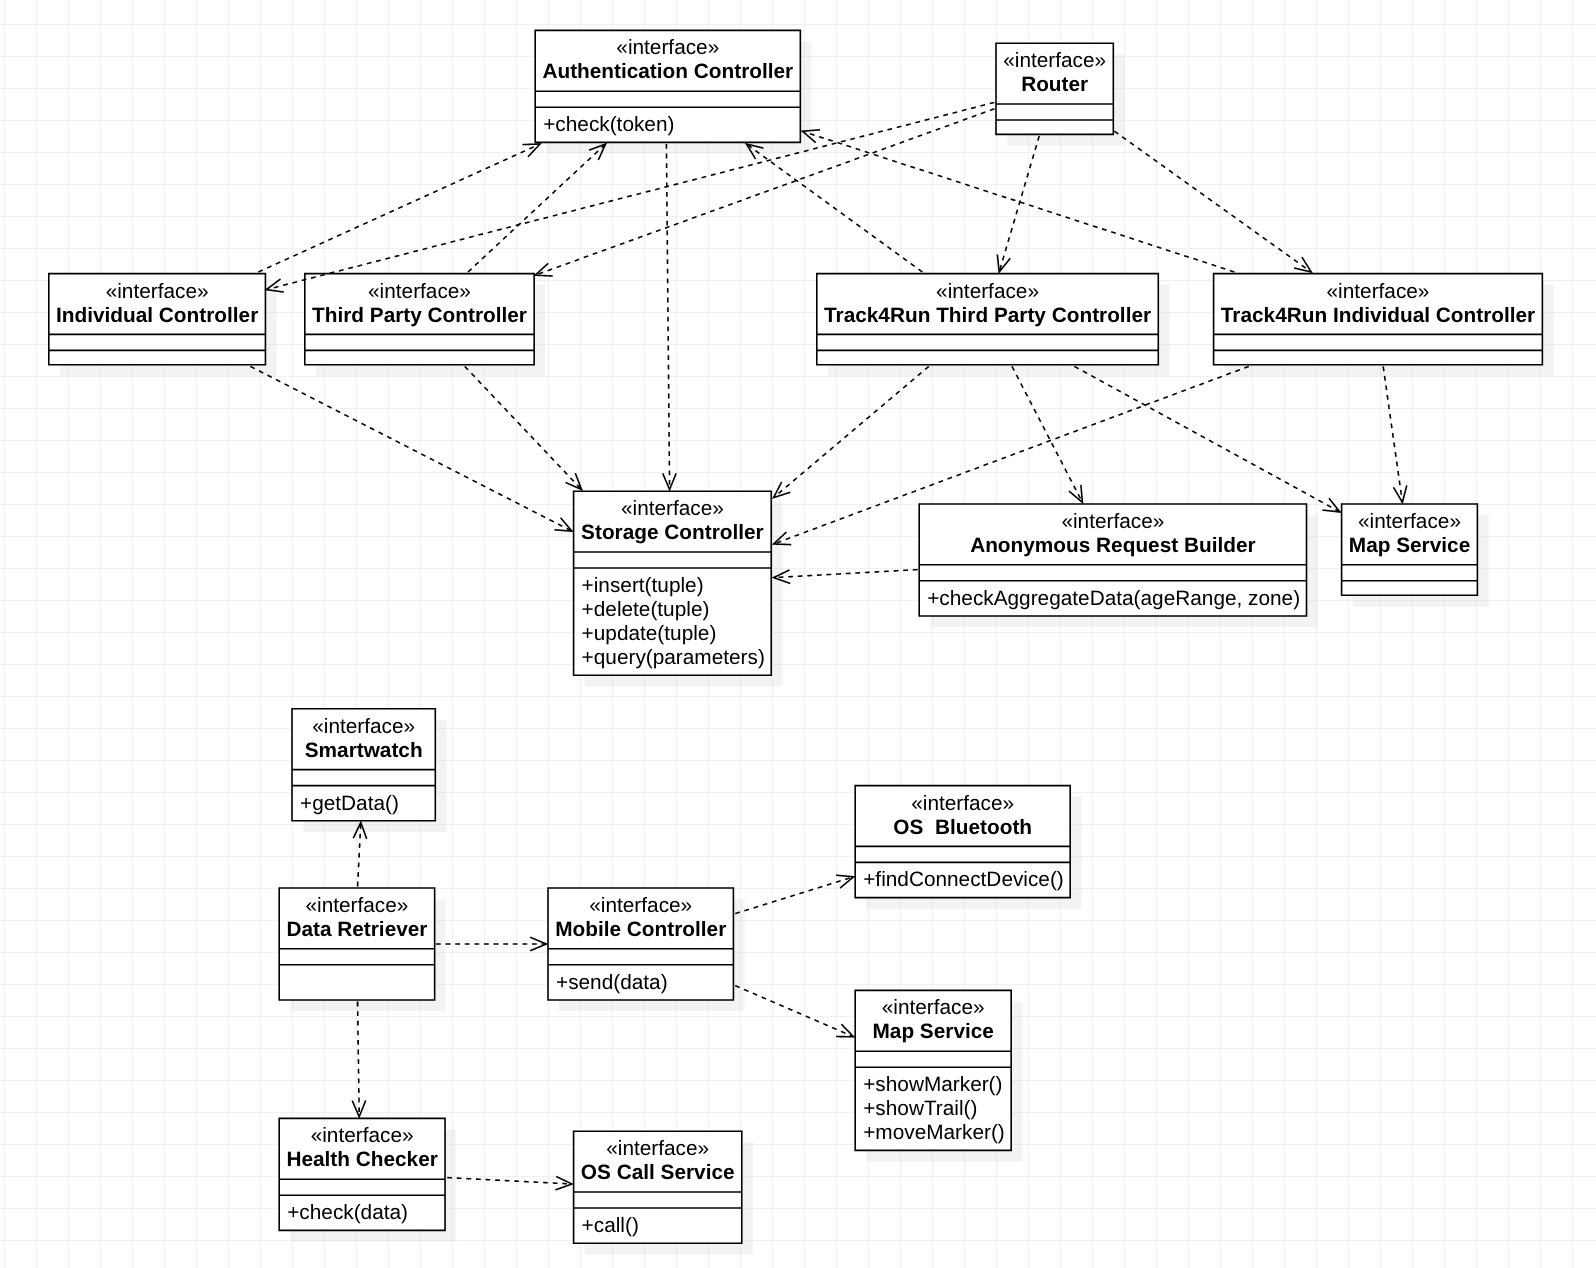
\includegraphics[width=\linewidth]{../images/design/interfaces.png}
						\end{figure} 
				\end{legal}
		\newpage
		\item \textit{\textbf{Selected architectural styles and patterns}}\\\\
			\begin{legal}
				\item \textit{\textbf{Multitier architecture}}\\\\
				TrackMe is built as a multitier architecture. More precisely it's a client/server architecture in which presentation, application processing, and data management functions are physically separated. 
				\begin{itemize}
					\item Presentation tier: provides basic user interface and application access services.
					\item Application processing tier: contains business logic and controls application functionalities.
					\item Data management tier: provides the mechanism used to access and process data and holds and manages data.
				\end{itemize}
				 This division allows each tier to be separately developed, tested, executed and reused. Other benefits of such architecture are scalability, ease of management, flexibility, and security.
				\begin{itemize}
					\item Secure: You can secure each of the three tiers separately using different methods.
					\item Easy to manage: You can manage each tier separately, adding or modifying each tier without affecting the other tiers.
					\item Scalable: If you need to add more resources, you can do it per tier, without affecting the other tiers.
					\item Flexible: Apart from isolated scalability, you can also expand each tier in any manner that your requirements dictate.\\
				\end{itemize}
				\item \textit{\textbf{Hybrid Client}}\\\\
				In our system presentation and application processing are not really totally separated, because mobile client applications have got components which work on the analysis and filtering of data. For this reason individual mobile applications are not thin clients. But they are not even considered as fat clients, because they are not thought to rely on a local store, so they are called hybrid clients. Furthermore, clients, included third parties machines, can't be considered thin clients because they have a local controller as explained in the next section.\\\\
				\item \textit{\textbf{MVC}}\\\\
				The main idea compared to other more traditional server-side architectures is to build the server as a set of stateless reusable REST services, and from an MVC perspective to take the controller out of the backend and move it into the client.
				The client is MVC-capable and contains all the presentation logic which is separated in a view layer, a controller layer, and a frontend services layer. After the initial application startup, only JSON data go over the wire between client and server.
				The frontend should only handle presentation logic, but no business logic. These are the three layers of the frontend:
				\begin{itemize}
					\item The view layer: it's intended to be displayed to the user. The presentation contains not just the content, but also the attributes for display such as HTML and CSS.
					\item The controller layer: it's made of functions that glue the data retrieved from the backend and the view together. The controller initialises the view model and defines how the view should react to model changes and vice-versa.
					\item The frontend services layer: a set of functions that allow to interact with the backend and with the controller layer.
				\end{itemize}
				The backend is built using the usual backend layers:
				\begin{itemize}
    				\item Router layer: it defines which service entry points correspond to a given HTTP URL, and how parameters have to be read from the HTTP request.
					\item Controller Layer: it contains any business logic such as validations, defines the scope of business transactions. Business rules are centralized into this business logic layer that serves as an intermediary for data exchange between the front-end layer and the persistence (storage controller) layer.
    				\item Storage controller layer: maps the database to/from in-memory domain objects.
				\end{itemize}
				\begin{figure}
			  		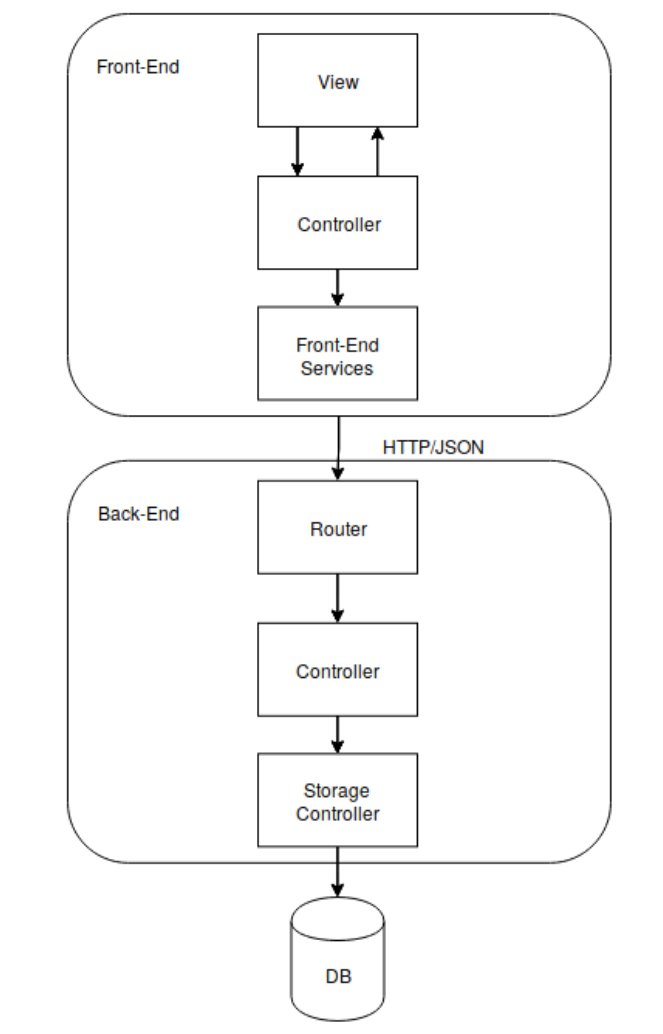
\includegraphics[width=\linewidth]{../images/design/MVC.png}
				\end{figure} 
				
			\end{legal}
			
  	\end{legal}
